% The contents of this file is 
% Copyright (c) 2009-2011  Charles R. Severance, All Righs Reserved

%\documentclass[10pt,b5paper]{book}
\documentclass[11pt]{book}
% \usepackage[width=5.25in,height=7.50in,hmarginratio=3:2,vmarginratio=1:1]{geometry}
\usepackage[size=journal,gutter=0.75in,trim,bleed]{createspace}

\usepackage[utf8]{inputenc}
\usepackage{pslatex}
\usepackage{url}
\usepackage{fancyhdr}
\usepackage{graphicx}
\usepackage{amsmath, amsthm, amssymb}
\usepackage{exercise}
\usepackage{makeidx}
\usepackage{setspace}
\usepackage{hevea}
\usepackage{alltt}
\usepackage{upquote}
%\usepackage{pslatex}
%\usepackage{url}
%\usepackage{fancyhdr}
%\usepackage{graphicx}
%\usepackage{amsmath, amsthm, amssymb}
%\usepackage{exercise}
%\usepackage{makeidx}
%\usepackage{setspace}
%\usepackage{hevea}
%\usepackage{alltt}
%\usepackage{upquote}

\usepackage[brazilian]{babel}

\newcommand{\thetitle}{Python para Informáticos: Explorando a Informação}
\newcommand{\theversion}{2.7.2}
%\newcommand{\thetitle}{Python for Informatics: Exploring Information}
%\newcommand{\theversion}{2.7.2}

\makeindex

\begin{document}

\frontmatter

% The contents of this file is 
% Copyright (c) 2009-  Charles R. Severance, All Righs Reserved

% LATEXONLY

\input{latexonly}

\def\exercisename{Exercício}

\newtheorem{ex}{\exercisename}[chapter]

\begin{latexonly}

\renewcommand{\blankpage}{\thispagestyle{empty} \quad \newpage}

\thispagestyle{empty}

\begin{flushright}
\vspace*{2.0in}

\begin{spacing}{3}
{\huge Python para Informáticos}\\
{\Large Explorando a Informação}
\end{spacing}
%\begin{spacing}{3}
%{\huge Python for Informatics}\\
%{\Large Exploring Information}
%\end{spacing}

\vspace{0.25in}

Version \theversion

\vspace{0.5in}


{\Large
Autor: Charles Severance\\
Tradução: @victorjabur
}
%{\Large
%Charles Severance\\
%}

\vfill

\end{flushright}

%--copyright--------------------------------------------------
\pagebreak
\thispagestyle{empty}

{\small
Copyright \copyright ~2009- Charles Severance.
Tradução: PT-BR \copyright ~2015- : @victorjabur
%{\small
%Copyright \copyright ~2009- Charles Severance.

Histórico de Publicação:
%Printing history:

\begin{description}

\item[Maio 2015:] Checagem editorial obrigado a Sue Blumenberg.
%\item[May 2015:] Editorial pass thanks to Sue Blumenberg.

\item[Outubro 2013:] Revisão principal dos Capítulos 13 e 14
para mudar para JSON e usar OAuth.
Novo capítulo adicionado na Visualização.
%\item[October 2013:] Major revision to Chapters 13 and 14
%to switch to JSON and use OAuth.
%Added new chapter on Visualization.

\item[Setembro 2013:] Livro publicado na Amazon CreateSpace
%\item[September 2013:] Published book on Amazon CreateSpace

\item[Janeiro 2010:] Livro publicado usando a máquina da Universidade de 
Michigan Espresso Book.
%\item[January 2010:] Published book using the University of 
%Michigan Espresso Book machine.

\item[Dezembro 2009:] Revisão principal dos capítulos 2-10 de
\emph{Think Python: How to Think Like
a Computer Scientist}
e escrita dos capítulos 1 e 11-15 para
produzir 
\emph{Python for Informatics: Exploring Information}
%\item[December 2009:] Major revision to chapters 2-10 from
%\emph{Think Python: How to Think Like
%a Computer Scientist}
%and writing chapters 1 and 11-15 to
%produce 
%\emph{Python for Informatics: Exploring Information}

\item[Junho 2008:] Revisão prncipal, título alterado para
\emph{Think Python: How to Think Like
a Computer Scientist}.
%\item[June 2008:] Major revision, changed title to
%\emph{Think Python: How to Think Like
%a Computer Scientist}.

\item[Agosto 2007:] Revisão principal, título alterado para
\emph{How to Think Like a (Python) Programmer}.
%\item[August 2007:] Major revision, changed title to
%\emph{How to Think Like a (Python) Programmer}.

\item[Abril 2002:] Primeira edição de \emph{How to Think Like
a Computer Scientist}.
%\item[April 2002:] First edition of \emph{How to Think Like
%a Computer Scientist}.

\end{description}

\vspace{0.2in}

Este trabalho está licenciado sob a 
Creative Common
Attribution-NonCommercial-ShareAlike 3.0 licença não portada.
Esta licença está
disponível em
\url{creativecommons.org/licenses/by-nc-sa/3.0/}.  Você pode 
ver as considerações nas quais o autor considera a utilização comercial e não comercial
deste material assim como as exceções da licença
no apêndice entitulado Detalhes dos Direitos Autorais.
%This work is licensed under a 
%Creative Common
%Attribution-NonCommercial-ShareAlike 3.0 Unported License.
%This license is 
%available at
%\url{creativecommons.org/licenses/by-nc-sa/3.0/}.  You can 
%see what the author considers commercial and non-commercial
%uses of this material as well as license exemptions 
%in the Appendix titled Copyright Detail.

O código fonte \LaTeX\ para a 
\emph{Think Python: How to Think Like
a Computer Scientist}
versão deste livro está disponível em
\url{http://www.thinkpython.com}.
%The \LaTeX\ source for the 
%\emph{Think Python: How to Think Like
%a Computer Scientist}
%version of this book is available from
%\url{http://www.thinkpython.com}.

\vspace{0.2in}

} % end small

\end{latexonly}


% HTMLONLY

\begin{htmlonly}

% TITLE PAGE FOR HTML VERSION

{\Large \thetitle}

{\large 
Charles Severance}

Version \theversion

\setcounter{chapter}{-1}

\end{htmlonly}

% The contents of this file is 
% Copyright (c) 2009- Charles R. Severance, All Righs Reserved

\chapter{Prefácio}
%\chapter{Preface}

\section*{Python para Informáticos: Adaptação de um livro aberto}
%\section*{Python for Informatics: Remixing an Open Book}

É muito comum que acadêmicos, em sua profissão, necessitem publicar continuamente 
materiais ou artigos quando querem criar algo do zero. 
Este livro é um experimento em não partir da estaca zero, mas sim ``remixar''
o livro entitulado \emph{Think Python: How to Think Like
a Computer Scientist} escrito por Allen B. Downey, Jeff Elkner, e outros.
%It is quite natural for academics who are continuously told to 
%``publish or perish'' to want to always create something from scratch
%that is their own fresh creation.   This book is an 
%experiment in not starting from scratch, but instead ``remixing''
%the book titled
%\emph{Think Python: How to Think Like
%a Computer Scientist}
%written by Allen B. Downey, Jeff Elkner, and others.

Em dezembro de 2009, quando estava me preparando para ministrar a disciplina
{\bf SI502 - Programação para Redes} na Universidade de Michigan
para o quinto semestre e decidi que era hora de escrever um livro de Python 
focado em explorar dados ao invés de entender algoritmos e 
abstrações.
Minha meta em SI502 é ensinar pessoas a terem habilidades na manipulação de dados 
para a vida usando Python.  Alguns dos meus estudantes estavam planejando tornarem-se 
profissionais em programação de computadores.  Ao invés disso, eles
escolheram ser bibliotecários, gerentes, advogados, biólogos, economistas, etc., 
e preferiram utilizar habilmente a tecnologia nas áreas de suas escolhas.
%In December of 2009, I was preparing to teach
%{\bf SI502 - Networked Programming} at the University of Michigan
%for the fifth semester in a row and decided it was time
%to write a Python textbook that focused on exploring data
%instead of understanding algorithms and abstractions.
%My goal in SI502 is to teach people lifelong data handling 
%skills using Python.  Few of my
%students were planning to be professional 
%computer programmers.  Instead, they
%planned to be librarians, managers, lawyers, biologists, economists, etc., 
%who happened to want to skillfully use technology in their chosen field.

Eu nunca consegui encontrar o livro perfeito sobre Python que fosse orientado a dados
para utilizar no meu curso, então eu comecei a escrever o meu próprio. Com muita sorte, em 
uma reunião eventual três semanas antes de eu começar a escrever o meu novo livro do zero, 
em um descanso no feriado, Dr. Atul Prakash me mostrou o \emph{Think Python} livro que ele tinha
usado para ministrar seu Curso de Python naquele semestre.
Era um texto muito bem escrito sobre Ciência da Computação com foco em
explicações diretas e simples de se aprender.
%I never seemed to find the perfect data-oriented Python
%book for my course, so I set out 
%to write just such a book.  Luckily at a faculty meeting three weeks
%before I was about to start my new book from scratch over 
%the holiday break, 
%Dr. Atul Prakash showed me the \emph{Think Python} book which he had
%used to teach his Python course that semester.  
%It is a well-written Computer Science text with a focus on 
%short, direct explanations and ease of learning. 

Toda a estrutura do livro foi alterada, visando a resolução de problemas de análise de 
dados de um modo tão simples e rápido quanto possível, acrescido de uma série de exemplos 
executáveis e exercícios sobre análise de dados desde o início.
%The overall book structure
%has been changed to get to doing data analysis problems as quickly as
%possible and have a series of running examples and exercises 
%about data analysis from the very beginning.  

Os capítulos 2--10 são similares ao livro \emph{Think Python}
mas precisaram de muitas alterações. Exemplos com numeração e
exercícios foram substituídos por exercícios orientados a dados.
Tópicos foram apresentados na ordem necessária para construir
soluções sofisticadas em análise de dados. Alguns tópicos tais como {\tt try}
e {\tt except} foram movidos mais para o final e apresentados como parte do
capítulo de condicionais. Funções foram necessárias para simplificar
a complexidade na manipulação dos programas introduzidos anteriormente
nas primeiras lições em abstração. Quase todas as funções definidas pelo usuário
foram removidas dos exemplos do código e exercícios, com exceção do Capítulo 4.
A palavra ``recursão''\footnote{Com exceção, naturalmente, desta linha.}
não aparece no livro inteiro.
%Chapters 2--10 are similar to the \emph{Think Python} book,
%but there have been major changes. Number-oriented examples and
%exercises have been replaced with data-oriented exercises.
%Topics are presented in the order needed to build increasingly
%sophisticated data analysis solutions. Some topics like {\tt try} and
%{\tt except} are pulled forward and presented as part of the chapter
%on conditionals.  Functions are given very light treatment until 
%they are needed to handle program complexity rather than introduced 
%as an early lesson in abstraction.  Nearly all user-defined functions
%have been removed from the example code and exercises outside of Chapter 4.
%The word ``recursion''\footnote{Except, of course, for this line.}
%does not appear in the book at all.

Nos capítulos 1 e 11--16, todo o material é novo, focado
em exemplos reais de uso e exemplos simples de Python para análise de dados
incluindo expressões regulares para busca e transformação,
automação de tarefas no seu computador, recuperação de dados na internet,
extração de dados de páginas web, utilização de web services, transformação
de dados em XML para JSON, e a criação e utilização de bancos de dados utilizando
SQL (Linguagem estruturada de consulta em bancos de dados).
%In chapters 1 and 11--16, all of the material is brand new, focusing
%on real-world uses and simple examples of Python for data analysis 
%including regular expressions for searching and parsing, 
%automating tasks on your computer, retrieving data across 
%the network, scraping web pages for data, 
%using web services, parsing XML and JSON data, and creating 
%and using databases using Structured Query Language.

O último objetivo de todas estas alterações é a mudança de foco, de
Ciência da Computação para uma Informática que inclui somente tópicos
que podem ser utilizados em uma turma de primeira viagem (iniciantes) que
podem ser úteis mesmo se a escolha deles não for seguir uma carreira
profissional em programação de computadores.
%The ultimate goal of all of these changes is a shift from a 
%Computer Science to an Informatics
%focus is to only include topics into a first technology 
%class that can be useful even if one chooses not to 
%become a professional programmer.

Estudantes que acharem este livro interessante e quiserem se aprofundar
devem olhar o livro de Allen B. Downey's \emph{Think Python}. Porque há
muita sinergia entre os dois livros, estudantes irão rapidamente desenvolver
habilidades na área com a técnica de programação e o pensamento
em algoritmos, que são cobertos em \emph{Think Python}.
Os dois livros possuem um estilo de escrita similar, é possível
mover-se para o livro \emph{Think Python} com o mínimo de esforço.
%Students who find this book interesting and want to further explore
%should look at Allen B. Downey's \emph{Think Python} book.  Because there
%is a lot of overlap between the two books,
%students will quickly pick up skills in the additional
%areas of technical programming and algorithmic thinking 
%that are covered in \emph{Think Python}.
%And given that the books have a similar writing style, they should be 
%able to move quickly through \emph{Think Python} with a minimum of effort.

\index{Creative Commons License}
\index{CC-BY-SA}
\index{BY-SA}
Com os direitos autorais de \emph{Think Python},
Allen me deu permissão para trocar a licença do livro
em relação ao livro no qual este material é baseado de 
GNU Licença Livre de Documentação para a mais recente
Creative Commons Attribution --- Licença de compartilhamento sem 
ciência do autor.
Esta baseia-se na documentação aberta de licenças mudando da GFDL
para a CC-BY-SA (i.e., Wikipedia).
Usando a licença CC-BY-SA, os mantenedores deste livro recomendam
fortemente a tradição ``copyleft'' que incentiva os novos autores
a reutilizarem este material da forma como considerarem adequada.

%\index{Creative Commons License}
%\index{CC-BY-SA}
%\index{BY-SA}
%As the copyright holder of \emph{Think Python},
%Allen has given me permission to change the book's license 
%on the material from his book that remains in this book
%from the
%GNU Free Documentation License 
%to the more recent
%Creative Commons Attribution --- Share Alike
%license.
%This follows a general shift in open documentation licenses moving 
%from the GFDL to the CC-BY-SA (e.g., Wikipedia).
%Using the CC-BY-SA license maintains the book's 
%strong copyleft tradition while making it even more straightforward 
%for new authors to reuse this material as they see fit.

Eu sinto que este livro serve de exemplo sobre como materiais
abertos (gratuitos) são importantes para o futuro da educação,
e quero agradecer ao Allen B. Downey e à editora da Universidade de 
Cambridge por sua decisão de tornar este livro disponível sob uma licença
aberta de direitos autorais. Eu espero que eles fiquem satisfeitos com
os resultados dos meus esforços e eu desejo que você leitor esteja satisfeito
com \emph{nosso} esforço coletivo.
%I feel that this book serves an example of why open 
%materials are so important to the future of education,
%and want to thank Allen B. Downey and Cambridge University
%Press for their forward-looking decision to make the book available
%under an open copyright.   I hope they are pleased with the 
%results of my efforts and I hope that you the reader are pleased with
%\emph{our} collective efforts.

Eu quero fazer um agradecimento ao Allen B. Downey e Lauren Cowles por sua ajuda,
paciência, e instrução em lidar com este trabalho e resolver os problemas de 
direitos autorais que cercam este livro.
%I would like to thank Allen B. Downey and Lauren Cowles for their help,
%patience, and guidance in dealing with and resolving the copyright 
%issues around this book.

Charles Severance\\
www.dr-chuck.com\\
Ann Arbor, MI, USA\\
9 de Setembro de 2013
%Charles Severance\\
%www.dr-chuck.com\\
%Ann Arbor, MI, USA\\
%September 9, 2013

Charles Severance é um 
Professor Associado 
à Escola de Informação da Universidade de Michigan.
%Charles Severance is a 
%Clinical Associate Professor 
%at the University of Michigan School of Information.

Tradução:\\
@victorjabur

\clearemptydoublepage

% TABLE OF CONTENTS
\begin{latexonly}

\tableofcontents

\clearemptydoublepage

\end{latexonly}

% START THE BOOK
\mainmatter



% START THE BOOK
\mainmatter

% The contents of this file is 
% Copyright (c) 2009-  Charles R. Severance, All Righs Reserved

\chapter{Por que você deve aprender a escrever programas ?}
%\chapter{Why should you learn to write programs?}

Escrever programas (ou programação) é uma atividade
muito criativa e recompensadora. Você pode escrever programas por
muitas razões, que vão desde resolver um difícil problema de 
análise de dados a se divertir ajudando alguém a resolver um
problema. Este livro assume que \emph{qualquer pessoa} precisa
saber como programar, e uma vez que você sabe como programar,
você irá imaginar o que você quer fazer com suas novas habilidades.
%Writing programs (or programming) is a very creative 
%and rewarding activity.  You can write programs for 
%many reasons, ranging from making your living to solving
%a difficult data analysis problem to having fun to helping
%someone else solve a problem.  This book assumes that 
%\emph{everyone} needs to know how to program, and that once 
%you know how to program you will figure out what you want 
%to do with your newfound skills.

Nós estamos cercados no nosso dia a dia por computadores, desde
notebooks até celulares. Nós podemos achar que estes computadores
são nossos ``assistentes pessoais'' que podem cuidar de muitas coisas
a nosso favor. O hardware desses computadores no nosso dia a dia é
essencialmente construído para nos responder a uma pergunta,
``O que você quer que eu faça agora ?''
%We are surrounded in our daily lives with computers ranging 
%from laptops to cell phones.  We can think of these computers
%as our ``personal assistants'' who can take care of many things
%on our behalf.  The hardware in our current-day computers 
%is essentially built to continuously ask us the question, 
%``What would you like me to do next?''

\beforefig
\centerline{\includegraphics[height=1.00in]{figs2/pda.eps}}
\afterfig

Programadores adicionam um sistema operacional e um conjunto de
aplicações ao hardware e nós terminamos com um Assistente 
Pessoal Digital que é muito útil e capaz de nos ajudar a fazer
diversas coisas.
%Programmers add an operating system and a set of applications
%to the hardware and we end up with a Personal Digital
%Assistant that is quite helpful and capable of helping
%us do many different things.

Nossos computadores são rápidos, tem vasta quantidade de memória
e pode ser muito útil para nós, somente se conhecermos a linguagem
falada para explicar para um computador o que nós gostaríamos
de fazer ``em seguida''. Se nós conhecemos esta linguagem, nós
podemos pedir ao computador para fazer tarefas repetitivas a 
nosso favor. Curiosamente, as coisas que os computadores
podem fazer melhor são frequentemente aquelas coisas que humanos
acham chatas e entediantes.
%Our computers are fast and have vast amounts of memory and 
%could be very helpful to us if we only knew the language to
%speak to explain to the computer what we would like it to 
%``do next''.  If we knew this language, we could tell the 
%computer to do tasks on our behalf that were repetitive.  
%Interestingly, the kinds of things computers can do best
%are often the kinds of things that we humans find boring
%and mind-numbing.

Por exemplo, olhe para os três primeiros parágrafos deste
capítulo e me diga qual é a palavra mais usada e quantas 
vezes. Contá-las é muito doloroso porque 
não é o tipo de problema que mentes humanas foram feitas para 
resolver. Para um computador o oposto é verdade, ler e entender o texto
de um pedaço de papel é difícil, mas contar palavras dizendo a 
você quantas vezes ela aparece é muito fácil:
%For example, look at the first three paragraphs of this
%chapter and tell me the most commonly used word and how
%many times the word is used.  While you were able to read
%and understand the words in a few seconds, counting them
%is almost painful because it is not the kind of problem 
%that human minds are designed to solve.  For a computer
%the opposite is true, reading and understanding text 
%from a piece of paper is hard for a computer to do 
%but counting the words and telling you how many times
%the most used word was used is very easy for the
%computer:

\beforeverb
\begin{verbatim}
python palavras.py
Digite o nome do arquivo: palavras.txt
para 16
\end{verbatim}
\afterverb
%\beforeverb
%\begin{verbatim}
%python words.py
%Enter file:words.txt
%to 16
%\end{verbatim}
%\afterverb

Nosso ``assistente de análise pessoal de informações'' rapidamente
conta para nós que a palavra ``para'' foi utilizada dezesseis vezes nos
primeiros três parágrafos deste capítulo.
%Our ``personal information analysis assistant'' quickly 
%told us that the word ``to'' was used sixteen times in the
%first three paragraphs of this chapter.

Este fato de que os computadores são bons em coisas
que humanos não são é a razão pela qual você precisa tornar-se
qualificado em falar a ``linguagem do computador''. Uma vez
que você aprende esta nova linguagem, pode delegar tarefas
mundanas para o seu parceiro (o computador), ganhando mais tempo
para fazer coisas que você foi especialmente adaptado para fazer. Você agrega
criatividade, intuição e originalidade para o seu parceiro. 
%This very fact that computers are good at things 
%that humans are not is why you need to become
%skilled at talking ``computer language''.  Once you learn
%this new language, you can delegate mundane tasks
%to your partner (the computer), leaving more time 
%for you to do the 
%things that you are uniquely suited for.  You bring 
%creativity, intuition, and inventiveness to this
%partnership. 

\section{Criatividade e motivação}
%\section{Creativity and motivation}


Embora este livro não se destine a programadores profissionais, programação
profissional pode ser um trabalho muito gratificante, tanto financeiramente
quanto pessoalmente. Construir programas úteis, elegantes, inteligentes para
que outros utilizem é uma atividade criativa. Seu computador ou assistente
pessoal digital (PDA) geralmente contém muitos programas diferentes feitos por
diversos grupos de programadores, todos competindo por sua atenção e seu 
interesse. Eles tentam dar o seu melhor para atender suas necessidades e dar a
você uma boa experiência de usabilidade no processo. Em algumas situações,
quando você executa um trecho de software, os programadores são diretamente
recompensados por sua escolha.
%While this book is not intended for professional programmers, professional
%programming can be a very rewarding job both financially and personally.
%Building useful, elegant, and clever programs for others to use is a very
%creative activity.  Your computer or Personal Digital Assistant (PDA) 
%usually contains many different programs from many different groups of 
%programmers, each competing for your attention and interest.  They try 
%their best to meet your needs and give you a great user experience in the
%process.   In some situations, when you choose a piece of software, the 
%programmers are directly compensated because of your choice.

Se nós pensarmos em programas como resultado criativo de grupos de programadores,
então talvez a figura a seguir seja uma versão mais sensata de nosso PDA:
%If we think of programs as the creative output of groups of programmers,
%perhaps the following figure is a more sensible version of our PDA:

\beforefig
\centerline{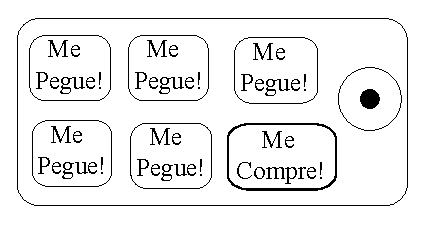
\includegraphics[height=1.00in]{figs2/pda2.eps}}
\afterfig

Por enquanto, nossa motivação primária não é ganhar dinheiro ou agradar usuários finais,
para nós sermos mais produtivos na manipulação de dados e informações
que nós encontraremos em nossas vidas.
Quando você começar, você será tanto o programador quanto o usuário final de seus
programas. Conforme você ganhar habilidades como programador e melhorar a criatividade
em seus próprios programas, mais você pode pensar em programar para os outros.
%For now, our primary motivation is not to make money or please end users, but
%instead for us to be more productive in handling the data and 
%information that we will encounter in our lives.
%When you first start, you will be both the programmer and the end user of
%your programs.  As you gain skill as a programmer and
%programming feels more creative to you, your thoughts may turn
%toward developing programs for others.
%

\section{Arquitetura física do Computador - Hardware}
\index{hardware}
\index{hardware!architecture}
%\section{Computer hardware architecture}
%\index{hardware}
%\index{hardware!architecture}
%

Antes de começar a estudar a linguagem, nós falamos
em dar instruções aos computadores para desenvolver software,
nós precisamos aprender um pouco mais sobre como os computadores
são construídos. Se você desmontar seu computador ou celular e olhar
por dentro, você encontrará as seguintes partes:
%Before we start learning the language we 
%speak to give instructions to computers to 
%develop software, we need to learn a small amount about 
%how computers are built.  If you were to take
%apart your computer or cell phone and look deep
%inside, you would find the following parts:
%

\beforefig
\centerline{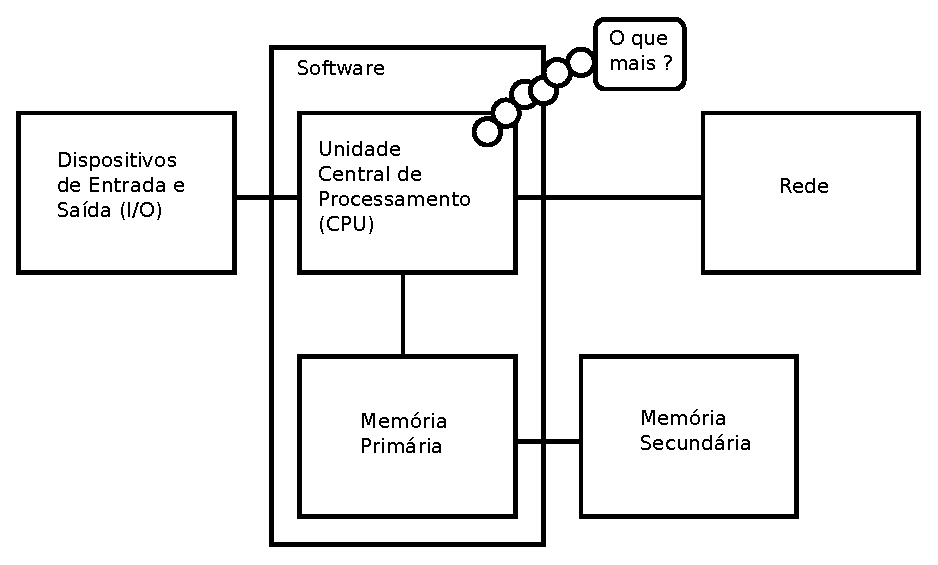
\includegraphics[height=2.50in]{figs2/arch.eps}}
\afterfig
%\beforefig
%\centerline{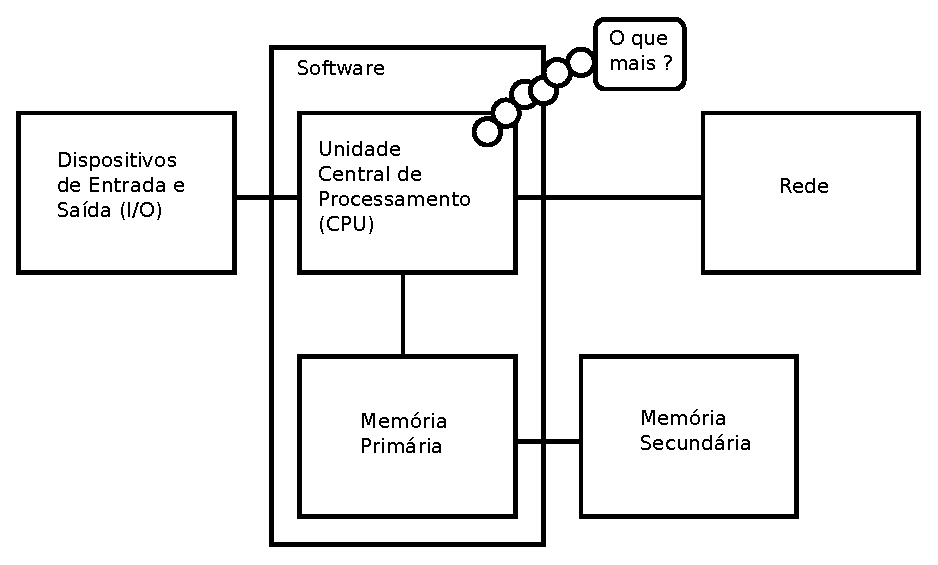
\includegraphics[height=2.50in]{figs2/arch.eps}}
%\afterfig
%

As definições resumidas destas partes são:
%The high-level definitions of these parts are as follows:
%

\begin{itemize}
%\begin{itemize}
%

\item A {\bf Unidade Central de Processamento} (ou CPU) é
a parte do computador que é feita para sempre te perguntar:
``O que mais ?'' Se seu computador possui uma frequência de
3.0 Gigahertz, significa que a CPU irá te perguntar ``O que mais ?''
três bilhões de vezes por segundo. Você irá aprender como conversar
tão rápido com a CPU.
%\item The {\bf Central Processing Unit} (or CPU) is 
%the part of the computer that is built to be obsessed 
%with ``what is next?''  If your computer is rated
%at 3.0 Gigahertz, it means that the CPU will ask ``What next?''
%three billion times per second.  You are going to have to 
%learn how to talk fast to keep up with the CPU.
%

\item A {\bf Memória Principal} é utilizada para armazenar informação
que a CPU precisa com muita pressa. A memória principal é aproximadamente
tão rápida quanto a CPU. Mas a informação armazenada na memória principal
se perde quando o computador é desligado (volátil).
%\item The {\bf Main Memory} is used to store information
%that the CPU needs in a hurry.  The main memory is nearly as 
%fast as the CPU.  But the information stored in the main
%memory vanishes when the computer is turned off.
%

\item A {\bf Memória Secundária} é também utilizada para armazenar
informação, mas ela é muito mais lenta que a memória principal.
A vantegem da memória secundária é que ela pode armazenar informação
que não se perde quando o computador é desligado. Exemplos de memória
secundária são discos rígidos (HD), pen drives, cartões de memória (sd card)
(tipicamente) encontradas no formato de USB e portáteis.
%\item The {\bf Secondary Memory} is also used to store
%information, but it is much slower than the main memory.
%The advantage of the secondary memory is that it can
%store information even when there is no power to the
%computer.  Examples of secondary memory are disk drives
%or flash memory (typically found in USB sticks and portable
%music players).
%

\item Os {\bf Dispositivos de Entrada e Saídas} são simplesmente
nosso monitor (tela), teclado, mouse, microfone, caixa de som, touchpad, etc.
Eles são todas as formas com as quais interagimos com o computador.
%\item The {\bf Input and Output Devices} are simply our
%screen, keyboard, mouse, microphone, speaker, touchpad, etc.  
%They are all of the ways we interact with the computer.
%

\item Atualmente, a maioria dos computadores tem uma
{\bf Conexão de Rede} para buscar informação em uma rede.
Nós podemos pensar a rede como um lugar muito lento para armazenar
e buscar dados que podem não estar ``disponíveis''. Em essência,
a rede é mais lenta e às vezes parece uma forma não confiável de
{\bf Memória Secundária}.
%\item These days, most computers also have a
%{\bf Network Connection} to retrieve information over a network.
%We can think of the network as a very slow place to store and
%retrieve data that might not always be ``up''.  So in a sense,
%the network is a slower and at times unreliable form of
%{\bf Secondary Memory}.
%

\end{itemize}
%\end{itemize}
%

É melhor deixar a maior parte dos detalhes de como estes componentes funcionam para
os construtores dos computadores, isso nos ajuda a ter alguma terminologia
que podemos utilizar para conversar sobre as diferentes partes nos programas
que vamos escrever.
%While most of the detail of how these components work is best left 
%to computer builders, it helps to have some terminology
%so we can talk about these different parts as we write our programs.
%

Como um programador, seu trabalho é usar e orquestrar
cada um destes recursos para resolver um problema que você precisa resolver
e analisar os dados que você obtém da solução. Como um programador você irá
``conversar'' com a CPU e contar a ela o que fazer em um próximo passo.
Algumas vezes você irá dizer à CPU para usar a memória principal, a memória
secundária, a rede ou os dispositivos de entrada e saída.
%As a programmer, your job is to use and orchestrate 
%each of these resources to solve the problem that you need to solve
%and analyze the data you get from the solution.  As a programmer you will 
%mostly be ``talking'' to the CPU and telling it what to 
%do next.  Sometimes you will tell the CPU to use the main memory,
%secondary memory, network, or the input/output devices.
%

\beforefig
\centerline{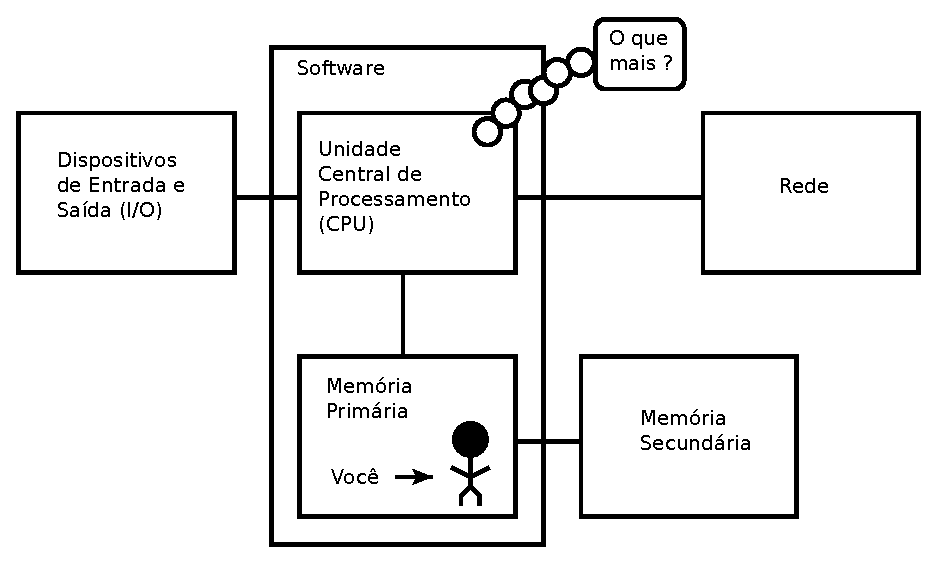
\includegraphics[height=2.50in]{figs2/arch2.eps}}
\afterfig
%\beforefig
%\centerline{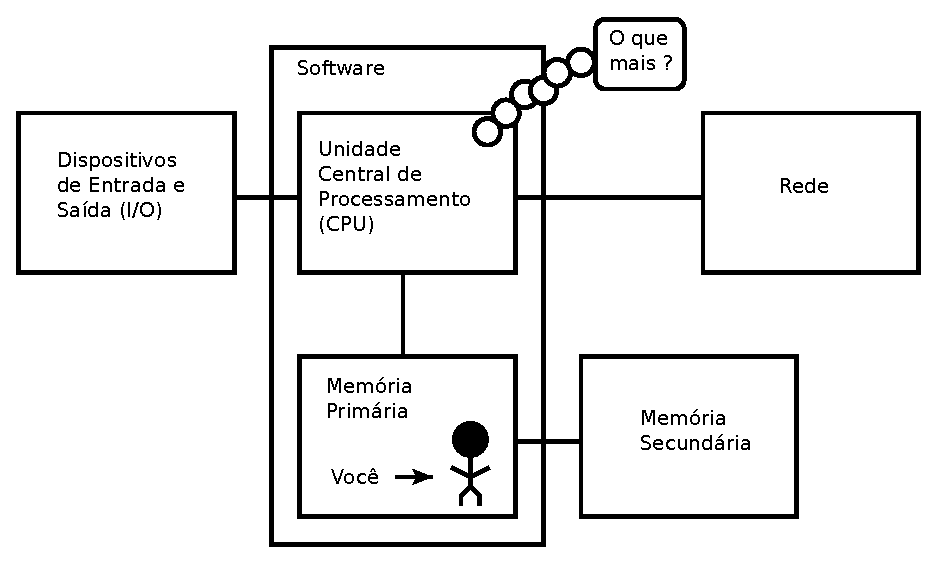
\includegraphics[height=2.50in]{figs2/arch2.eps}}
%\afterfig
%


%You need to be the person who answers the CPU's ``What next?'' 
%question.  But it would be very uncomfortable to shrink you 
%down to 5mm tall and insert you into the computer just so you 
%could issue a command three billion times per second.  So instead,
%you must write down your instructions in advance.
%We call these stored instructions a {\bf program} and the act 
%of writing these instructions down and getting the instructions to 
%be correct {\bf programming}.
%
%\section{Understanding programming}
%
%In the rest of this book, we will try to turn you into a person
%who is skilled in the art of programming.  In the end you will be a 
%{\bf programmer} --- perhaps not a professional programmer, but 
%at least you will have the skills to look at a data/information
%analysis problem and develop a program to solve the problem.
%
%\index{problem solving}
%
%In a sense, you need two skills to be a programmer:
%
%\begin{itemize}
%
%\item First, you need to know the programming language (Python) -
%you need to know the vocabulary and the grammar.  You need to be able 
%to spell the words in this new language properly and know how to construct 
%well-formed ``sentences'' in this new language.
%
%\item Second, you need to ``tell a story''.  In writing a story,
%you combine words and sentences to convey an idea to the reader. 
%There is a skill and art in constructing the story, and skill in
%story writing is improved by doing some writing and getting some
%feedback.  In programming, our program is the ``story'' and the 
%problem you are trying to solve is the ``idea''.
%
%\end{itemize}
%
%Once you learn one programming language such as Python, you will 
%find it much easier to learn a second programming language such
%as JavaScript or C++.  The new programming language has very different 
%vocabulary and grammar but the problem-solving skills 
%will be the same across all programming languages.
%
%You will learn the ``vocabulary'' and ``sentences'' of Python pretty quickly.
%It will take longer for you to be able to write a coherent program
%to solve a brand-new problem.  We teach programming much like we teach
%writing.  We start reading and explaining programs, then we write 
%simple programs, and then we write increasingly complex programs over time.
%At some point you ``get your muse'' and see the patterns on your own
%and can see more naturally how to take a problem and 
%write a program that solves that problem.  And once you get 
%to that point, programming becomes a very pleasant and creative process.  
%
%We start with the vocabulary and structure of Python programs.  Be patient
%as the simple examples remind you of when you started reading for the first
%time. 
%
%\section{Words and sentences}
%\index{programming language}
%\index{language!programming}
%
%Unlike human languages, the Python vocabulary is actually pretty small.
%We call this ``vocabulary'' the ``reserved words''.  These are words that
%have very special meaning to Python.  When Python sees these words in 
%a Python program, they have one and only one meaning to Python.  Later
%as you write programs you will make up your own words that have meaning to 
%you called {\bf variables}.   You will have great latitude in choosing
%your names for your variables, but you cannot use any of Python's 
%reserved words as a name for a variable.
%
%When we train a dog, we use special words like
%``sit'', ``stay'', and ``fetch''.  When you talk to a dog and
%don't use any of the reserved words, they just look at you with a 
%quizzical look on their face until you say a reserved word.  
%For example, if you say, 
%``I wish more people would walk to improve their overall health'', 
%what most dogs likely hear is,
%``blah blah blah {\bf walk} blah blah blah blah.''
%That is because ``walk'' is a reserved word in dog language.  Many
%might suggest that the language between humans and cats has no
%reserved words\footnote{\url{http://xkcd.com/231/}}.
%
%The reserved words in the language where humans talk to 
%Python include the following:
%
%\beforeverb
%\begin{verbatim}
%and       del       from      not       while    
%as        elif      global    or        with     
%assert    else      if        pass      yield    
%break     except    import    print              
%class     exec      in        raise              
%continue  finally   is        return             
%def       for       lambda    try
%\end{verbatim}
%\afterverb
%%
%That is it, and unlike a dog, Python is already completely trained.
%When you say ``try'', Python will try every time you say it without
%fail.
%
%We will learn these reserved words and how they are used in good time,
%but for now we will focus on the Python equivalent of ``speak'' (in 
%human-to-dog language).  The nice thing about telling Python to speak
%is that we can even tell it what to say by giving it a message in quotes:
%
%\beforeverb
%\begin{verbatim}
%print 'Hello world!'
%\end{verbatim}
%\afterverb
%
%And we have even written our first syntactically correct Python sentence.
%Our sentence starts with the reserved word {\bf print} followed
%by a string of text of our choosing enclosed in single quotes.
%
%\section{Conversing with Python}
%
%Now that we have a word and a simple sentence that we know in Python,
%we need to know how to start a conversation with Python to test 
%our new language skills.
%
%Before you can converse with Python, you must first install the Python
%software on your computer and learn how to start Python on your 
%computer.  That is too much detail for this chapter so I suggest
%that you consult \url{www.pythonlearn.com} where I have detailed
%instructions and screencasts of setting up and starting Python 
%on Macintosh and Windows systems.  At some point, you will be in 
%a terminal or command window and you will type {\bf python} and 
%the Python interpreter will start executing in interactive mode
%and appear somewhat as follows:
%\index{interactive mode}
%
%\beforeverb
%\begin{verbatim}
%Python 2.6.1 (r261:67515, Jun 24 2010, 21:47:49) 
%[GCC 4.2.1 (Apple Inc. build 5646)] on darwin
%Type "help", "copyright", "credits" or "license" for more information.
%>>> 
%\end{verbatim}
%\afterverb
%%
%The {\tt >>>} prompt is the Python interpreter's way of asking you, ``What
%do you want me to do next?''  Python is ready to have a conversation with
%you.  All you have to know is how to speak the Python language.
%
%Let's say for example that you did not know even the simplest Python language
%words or sentences. You might want to use the standard line that astronauts 
%use when they land on a faraway planet and try to speak with the inhabitants
%of the planet:
%
%\beforeverb
%\begin{verbatim}
%>>> I come in peace, please take me to your leader
%  File "<stdin>", line 1
%    I come in peace, please take me to your leader
%         ^
%SyntaxError: invalid syntax
%>>> 
%\end{verbatim}
%\afterverb
%%
%This is not going so well.  Unless you think of something quickly,
%the inhabitants of the planet are likely to stab you with their spears, 
%put you on a spit, roast you over a fire, and eat you for dinner.
%
%Luckily you brought a copy of this book on your travels, and you thumb to
%this very page and try again:
%
%\beforeverb
%\begin{verbatim}
%>>> print 'Hello world!'
%Hello world!
%\end{verbatim}
%\afterverb
%%
%This is looking much better, so you try to communicate some
%more:
%
%\beforeverb
%\begin{verbatim}
%>>> print 'You must be the legendary god that comes from the sky'
%You must be the legendary god that comes from the sky
%>>> print 'We have been waiting for you for a long time'
%We have been waiting for you for a long time
%>>> print 'Our legend says you will be very tasty with mustard'
%Our legend says you will be very tasty with mustard
%>>> print 'We will have a feast tonight unless you say
%  File "<stdin>", line 1
%    print 'We will have a feast tonight unless you say
%                                                     ^
%SyntaxError: EOL while scanning string literal
%>>> 
%\end{verbatim}
%\afterverb
%%
%The conversation was going so well for a while and then you
%made the tiniest mistake using the Python language and Python 
%brought the spears back out.
%
%At this point, you should also realize that while Python 
%is amazingly complex and powerful and very picky about 
%the syntax you use to communicate with it, Python is {\em 
%not} intelligent.  You are really just having a conversation
%with yourself, but using proper syntax.
%
%In a sense, when you use a program written by someone else
%the conversation is between you and those other
%programmers with Python acting as an intermediary.  Python
%is a way for the creators of programs to express how the 
%conversation is supposed to proceed.  And
%in just a few more chapters, you will be one of those
%programmers using Python to talk to the users of your program.
%
%Before we leave our first conversation with the Python 
%interpreter, you should probably know the proper way
%to say ``good-bye'' when interacting with the inhabitants
%of Planet Python:
%
%\beforeverb
%\begin{verbatim}
%>>> good-bye
%Traceback (most recent call last):
%  File "<stdin>", line 1, in <module>
%NameError: name 'good' is not defined
%
%>>> if you don't mind, I need to leave
%  File "<stdin>", line 1
%    if you don't mind, I need to leave
%             ^
%SyntaxError: invalid syntax
%
%>>> quit()
%\end{verbatim}
%\afterverb
%%
%You will notice that the error is different for the first two
%incorrect attempts.   The second error is different because 
%{\bf if} is a reserved word and Python saw the reserved word
%and thought we were trying to say something but got the syntax
%of the sentence wrong.
%
%The proper way to say ``good-bye'' to Python is to enter 
%{\bf quit()} at the interactive chevron {\tt >>>} prompt.
%It would have probably taken you quite a while to guess that 
%one, so having a book handy probably will turn out 
%to be helpful.
%
%\section{Terminology: interpreter and compiler}
%
%Python is a {\bf high-level} language intended to be relatively
%straightforward for humans to read and write and for computers
%to read and process.  Other high-level languages include Java, C++,
%PHP, Ruby, Basic, Perl, JavaScript, and many more.  The actual hardware
%inside the Central Processing Unit (CPU) does not understand any
%of these high-level languages.
%
%The CPU understands a language we call {\bf machine language}.  Machine
%language is very simple and frankly very tiresome to write because it 
%is represented all in zeros and ones:
%
%\beforeverb
%\begin{verbatim}
%01010001110100100101010000001111
%11100110000011101010010101101101
%...
%\end{verbatim}
%\afterverb
%%
%Machine language seems quite simple on the surface, given that there 
%are only zeros and ones, but its syntax is even more complex
%and far more intricate than Python.  So very few programmers ever write
%machine language.  Instead we build various translators to allow
%programmers to write in high-level languages like Python or JavaScript
%and these translators convert the programs to machine language for actual
%execution by the CPU.
%
%Since machine language is tied to the computer hardware, machine language
%is not {\bf portable} across different types of hardware.  Programs written in 
%high-level languages can be moved between different computers by using a 
%different interpreter on the new machine or recompiling the code to create
%a machine language version of the program for the new machine.
%
%These programming language translators fall into two general categories:
%(1) interpreters and (2) compilers.
%
%An {\bf interpreter} reads the source code of the program as written by the
%programmer, parses the source code, and interprets the instructions on the fly.
%Python is an interpreter and when we are running Python interactively, 
%we can type a line of Python (a sentence) and Python processes it immediately
%and is ready for us to type another line of Python.   
%
%Some of the lines of Python tell Python that you want it to remember some 
%value for later.   We need to pick a name for that value to be remembered and
%we can use that symbolic name to retrieve the value later.  We use the 
%term {\bf variable} to refer to the labels we use to refer to this stored data.
%
%\beforeverb
%\begin{verbatim}
%>>> x = 6
%>>> print x
%6
%>>> y = x * 7
%>>> print y
%42
%>>> 
%\end{verbatim}
%\afterverb
%%
%In this example, we ask Python to remember the value six and use the label {\bf x}
%so we can retrieve the value later.   We verify that Python has actually remembered
%the value using {\bf print}. Then we ask Python to retrieve {\bf x} and multiply
%it by seven and put the newly computed value in {\bf y}.  Then we ask Python to print out
%the value currently in {\bf y}.
%
%Even though we are typing these commands into Python one line at a time, Python
%is treating them as an ordered sequence of statements with later statements able
%to retrieve data created in earlier statements.   We are writing our first 
%simple paragraph with four sentences in a logical and meaningful order.
%
%It is the nature of an {\bf interpreter} to be able to have an interactive conversation
%as shown above.  A {\bf compiler} needs to be handed the entire program in a file, and then 
%it runs a process to translate the high-level source code into machine language
%and then the compiler puts the resulting machine language into a file for later
%execution.
%
%If you have a Windows system, often these executable machine language programs have a
%suffix of ``.exe'' or ``.dll'' which stand for ``executable'' and ``dynamic link
%library'' respectively.  In Linux and Macintosh, there is no suffix that uniquely marks
%a file as executable.
%
%If you were to open an executable file in a text editor, it would look 
%completely crazy and be unreadable:
%
%\beforeverb
%\begin{verbatim}
%^?ELF^A^A^A^@^@^@^@^@^@^@^@^@^B^@^C^@^A^@^@^@\xa0\x82
%^D^H4^@^@^@\x90^]^@^@^@^@^@^@4^@ ^@^G^@(^@$^@!^@^F^@
%^@^@4^@^@^@4\x80^D^H4\x80^D^H\xe0^@^@^@\xe0^@^@^@^E
%^@^@^@^D^@^@^@^C^@^@^@^T^A^@^@^T\x81^D^H^T\x81^D^H^S
%^@^@^@^S^@^@^@^D^@^@^@^A^@^@^@^A\^D^HQVhT\x83^D^H\xe8
%....
%\end{verbatim}
%\afterverb
%%
%It is not easy to read or write machine language, so it is nice that we have
%{\bf interpreters} and {\bf compilers} that allow us to write in high-level
%languages like Python or C.
%
%Now at this point in our discussion of compilers and interpreters, you should 
%be wondering a bit about the Python interpreter itself.  What language is 
%it written in?  Is it written in a compiled language?  When we type
%``python'', what exactly is happening?
%
%The Python interpreter is written in a high-level language called ``C''.  
%You can look at the actual source code for the Python interpreter by
%going to \url{www.python.org} and working your way to their source code.
%So Python is a program itself and it is compiled into machine code.
%When you installed Python on your computer (or the vendor installed it),
%you copied a machine-code copy of the translated Python program onto your
%system.   In Windows, the executable machine code for Python itself is likely
%in a file with a name like:
%
%\beforeverb
%\begin{verbatim}
%C:\Python27\python.exe
%\end{verbatim}
%\afterverb
%%
%That is more than you really need to know to be a Python programmer, but
%sometimes it pays to answer those little nagging questions right at 
%the beginning.
%
%\section{Writing a program}
%
%Typing commands into the Python interpreter is a great way to experiment 
%with Python's features, but it is not recommended for solving more complex problems.
%
%When we want to write a program, 
%we use a text editor to write the Python instructions into a file,
%which is called a {\bf script}.  By
%convention, Python scripts have names that end with {\tt .py}.
%
%\index{script}
%
%To execute the script, you have to tell the Python interpreter 
%the name of the file.  In a Unix or Windows command window, 
%you would type {\tt python hello.py} as follows:
%
%\beforeverb
%\begin{verbatim}
%csev$ cat hello.py
%print 'Hello world!'
%csev$ python hello.py
%Hello world!
%csev$
%\end{verbatim}
%\afterverb
%%
%The ``csev\$'' is the operating system prompt, and the ``cat hello.py'' is 
%showing us that the file ``hello.py'' has a one-line Python program to print
%a string.
%
%We call the Python interpreter and tell it to read its source code from
%the file ``hello.py'' instead of prompting us for lines of Python code
%interactively.
%
%You will notice that there was no need to have {\bf quit()} at the end of
%the Python program in the file.   When Python is reading your source code
%from a file, it knows to stop when it reaches the end of the file.
%
%\section{What is a program?}
%
%The definition of a {\bf program} at its most basic is a sequence
%of Python statements that have been crafted to do something.
%Even our simple {\bf hello.py} script is a program.  It is a one-line
%program and is not particularly useful, but in the strictest definition,
%it is a Python program.
%
%It might be easiest to understand what a program is by thinking about a problem 
%that a program might be built to solve, and then looking at a program
%that would solve that problem.
%
%Lets say you are doing Social Computing research on Facebook posts and 
%you are interested in the most frequently used word in a series of posts.
%You could print out the stream of Facebook posts and pore over the text
%looking for the most common word, but that would take a long time and be very 
%mistake prone.  You would be smart to write a Python program to handle the
%task quickly and accurately so you can spend the weekend doing something 
%fun.
%
%For example, look at the following text about a clown and a car.  Look at the 
%text and figure out the most common word and how many times it occurs.
%
%\beforeverb
%\begin{verbatim}
%the clown ran after the car and the car ran into the tent 
%and the tent fell down on the clown and the car 
%\end{verbatim}
%\afterverb
%%
%Then imagine that you are doing this task looking at millions of lines of 
%text.  Frankly it would be quicker for you to learn Python and write a 
%Python program to count the words than it would be to manually 
%scan the words.
%
%The even better news is that I already came up with a simple program to 
%find the most common word in a text file.  I wrote it,
%tested it, and now I am giving it to you to use so you can save some time.
%
%\beforeverb
%\begin{verbatim}
%name = raw_input('Enter file:')
%handle = open(name, 'r')
%text = handle.read()
%words = text.split()
%counts = dict()
%
%for word in words:
%   counts[word] = counts.get(word,0) + 1
%
%bigcount = None
%bigword = None
%for word,count in counts.items():
%    if bigcount is None or count > bigcount:
%        bigword = word
%        bigcount = count
%
%print bigword, bigcount
%\end{verbatim}
%\afterverb
%%
%You don't even need to know Python to use this program.  You will need to get through 
%Chapter 10 of this book to fully understand the awesome Python techniques that were
%used to make the program.  You are the end user, you simply use the program and marvel
%at its cleverness and how it saved you so much manual effort.
%You simply type the code 
%into a file called {\bf words.py} and run it or you download the source 
%code from \url{http://www.pythonlearn.com/code/} and run it.
%
%\index{program}
%This is a good example of how Python and the Python language are acting as an intermediary
%between you (the end user) and me (the programmer).  Python is a way for us to exchange useful
%instruction sequences (i.e., programs) in a common language that can be used by anyone who 
%installs Python on their computer.  So neither of us are talking {\em to Python},
%instead we are communicating with each other {\em through} Python.
%
%\section{The building blocks of programs}
%
%In the next few chapters, we will learn more about the vocabulary, sentence structure,
%paragraph structure, and story structure of Python.  We will learn about the powerful
%capabilities of Python and how to compose those capabilities together to create useful
%programs.
%
%There are some low-level conceptual patterns that we use to construct programs.  These
%constructs are not just for Python programs, they are part of every programming language
%from machine language up to the high-level languages.
%
%\begin{description}
%
%\item[input:] Get data from the ``outside world''.  This might be 
%reading data from a file, or even some kind of sensor like 
%a microphone or GPS.  In our initial programs, our input will come from the user
%typing data on the keyboard.
%
%\item[output:] Display the results of the program on a screen
%or store them in a file or perhaps write them to a device like a
%speaker to play music or speak text.
%
%\item[sequential execution:] Perform statements one after
%another in the order they are encountered in the script.
%
%\item[conditional execution:] Check for certain conditions and
%then execute or skip a sequence of statements.
%
%\item[repeated execution:] Perform some set of statements 
%repeatedly, usually with
%some variation.
%
%\item[reuse:] Write a set of instructions once and give them a name
%and then reuse those instructions as needed throughout your program.
%
%\end{description}
%
%It sounds almost too simple to be true, and of course it is never
%so simple.  It is like saying that walking is simply
%``putting one foot in front of the other''.  The ``art'' 
%of writing a program is composing and weaving these
%basic elements together many times over to produce something
%that is useful to its users.
%
%The word counting program above directly uses all of 
%these patterns except for one.
%
%\section{What could possibly go wrong?}
%
%As we saw in our earliest conversations with Python, we must
%communicate very precisely when we write Python code.  The smallest
%deviation or mistake will cause Python to give up looking at your
%program.
%
%Beginning programmers often take the fact that Python leaves no
%room for errors as evidence that Python is mean, hateful, and cruel.
%While Python seems to like everyone else, Python knows them 
%personally and holds a grudge against them.  Because of this grudge,
%Python takes our perfectly written programs and rejects them as 
%``unfit'' just to torment us.
%
%\beforeverb
%\begin{verbatim}
%>>> primt 'Hello world!'
%  File "<stdin>", line 1
%    primt 'Hello world!'
%                       ^
%SyntaxError: invalid syntax
%>>> primt 'Hello world'
%  File "<stdin>", line 1
%    primt 'Hello world'
%                      ^
%SyntaxError: invalid syntax
%>>> I hate you Python!
%  File "<stdin>", line 1
%    I hate you Python!
%         ^
%SyntaxError: invalid syntax
%>>> if you come out of there, I would teach you a lesson
%  File "<stdin>", line 1
%    if you come out of there, I would teach you a lesson
%              ^
%SyntaxError: invalid syntax
%>>> 
%\end{verbatim}
%\afterverb
%%
%There is little to be gained by arguing with Python.  It is just a tool.
%It has no emotions and it is happy and ready to serve you whenever you
%need it.  Its error messages sound harsh, but they are just Python's
%call for help.  It has looked at what you typed, and it simply cannot
%understand what you have entered.
%
%Python is much more like a dog, loving you unconditionally, having a few
%key words that it understands, looking you with a sweet look on its
%face ({\tt >>>}), and waiting for you to say something it understands.
%When Python says ``SyntaxError: invalid syntax'', it is simply wagging
%its tail and saying, ``You seemed to say something but I just don't
%understand what you meant, but please keep talking to me ({\tt >>>}).''
%
%As your programs become increasingly sophisticated, you will encounter three 
%general types of errors:
%
%\begin{description}
%
%\item[Syntax errors:] These are the first errors you will make and the easiest
%to fix.  A syntax error means that you have violated the ``grammar'' rules of Python.
%Python does its best to point right at the line and character where 
%it noticed it was confused.  The only tricky bit of syntax errors is that sometimes
%the mistake that needs fixing is actually earlier in the program than where Python
%{\em noticed} it was confused.  So the line and character that Python indicates in 
%a syntax error may just be a starting point for your investigation.
%
%\item[Logic errors:] A logic error is when your program has good syntax but there is a mistake 
%in the order of the statements or perhaps a mistake in how the statements relate to one another.
%A good example of a logic error might be, ``take a drink from your water bottle, put it 
%in your backpack, walk to the library, and then put the top back on the bottle.''
%
%\item[Semantic errors:] A semantic error is when your description of the steps to take 
%is syntactically perfect and in the right order, but there is simply a mistake in 
%the program.  The program is perfectly correct but it does not do what
%you {\em intended} for it to do. A simple example would
%be if you were giving a person directions to a restaurant and said, ``...when you reach
%the intersection with the gas station, turn left and go one mile and the restaurant
%is a red building on your left.''  Your friend is very late and calls you to tell you that
%they are on a farm and walking around behind a barn, with no sign of a restaurant.  
%Then you say ``did you turn left or right at the gas station?'' and 
%they say, ``I followed your directions perfectly, I have 
%them written down, it says turn left and go one mile at the gas station.''  Then you say,
%``I am very sorry, because while my instructions were syntactically correct, they 
%sadly contained a small but undetected semantic error.''. 
%
%\end{description}
%
%Again in all three types of errors, Python is merely trying its hardest to 
%do exactly what you have asked.
%
%\section{The learning journey}
%
%As you progress through the rest of the book, don't be afraid if the concepts 
%don't seem to fit together well the first time.  When you were learning to speak, 
%it was not a problem  for your first few years that you just made cute gurgling noises.
%And it was OK if it took six months for you to move from simple vocabulary to 
%simple sentences and took 5-6 more years to move from sentences to paragraphs, and a
%few more years to be able to write an interesting complete short story on your own.
%
%We want you to learn Python much more rapidly, so we teach it all at the same time
%over the next few chapters.  
%But it is like learning a new language that takes time to absorb and understand
%before it feels natural.
%That leads to some confusion as we visit and revisit
%topics to try to get you to see the big picture while we are defining the tiny
%fragments that make up that big picture.  While the book is written linearly, and
%if you are taking a course it will progress in a linear fashion, don't hesitate
%to be very nonlinear in how you approach the material.  Look forwards and backwards
%and read with a light touch.  By skimming more advanced material without 
%fully understanding the details, you can get a better understanding of the ``why?'' 
%of programming.  By reviewing previous material and even redoing earlier 
%exercises, you will realize that you actually learned a lot of material even 
%if the material you are currently staring at seems a bit impenetrable.
%
%Usually when you are learning your first programming language, there are a few
%wonderful ``Ah Hah!'' moments where you can look up from pounding away at some rock
%with a hammer and chisel and step away and see that you are indeed building 
%a beautiful sculpture.
%
%If something seems particularly hard, there is usually no value in staying up all 
%night and staring at it.   Take a break, take a nap, have a snack, explain what you 
%are having a problem with to someone (or perhaps your dog), and then come back to it with
%fresh eyes.  I assure you that once you learn the programming concepts in the book
%you will look back and see that it was all really easy and elegant and it simply 
%took you a bit of time to absorb it.
%
%\section{Glossary}
%
%\begin{description}
%
%\item[bug:]  An error in a program.
%\index{bug}
%
%\item[central processing unit:] The heart of any computer.  It is what
%runs the software that we write; also called ``CPU'' or ``the processor''.
%\index{central processing unit}
%\index{CPU}
%
%\item[compile:]  To translate a program written in a high-level language
%into a low-level language all at once, in preparation for later
%execution.
%\index{compile}
%
%\item[high-level language:]  A programming language like Python that
%is designed to be easy for humans to read and write.
%\index{high-level language}
%
%\item[interactive mode:] A way of using the Python interpreter by
%typing commands and expressions at the prompt.
%\index{interactive mode}
%
%\item[interpret:]  To execute a program in a high-level language
%by translating it one line at a time.
%\index{interpret}
%
%\item[low-level language:]  A programming language that is designed
%to be easy for a computer to execute; also called ``machine code'' or
%``assembly language''.
%\index{low-level language}
%
%\item[machine code:]  The lowest-level language for software, which 
%is the language that is directly executed by the central processing unit 
%(CPU).
%\index{machine code}
%
%\item[main memory:] Stores programs and data.  Main memory loses 
%its information when the power is turned off.
%\index{main memory}
%
%\item[parse:]  To examine a program and analyze the syntactic structure.
%\index{parse}
%
%\item[portability:]  A property of a program that can run on more
%than one kind of computer.
%\index{portability}
%
%\item[print statement:]  An instruction that causes the Python
%interpreter to display a value on the screen.
%\index{print statement}
%\index{statement!print}
%
%\item[problem solving:]  The process of formulating a problem, finding
%a solution, and expressing the solution.
%\index{problem solving}
%
%\item[program:] A set of instructions that specifies a computation.
%\index{program}
%
%\item[prompt:] When a program displays a message and pauses for the 
%user to type some input to the program.
%\index{prompt}
%
%\item[secondary memory:] Stores programs and data and retains its 
%information even when the power is turned off.  Generally slower 
%than main memory.  Examples of secondary memory include disk 
%drives and flash memory in USB sticks.
%\index{secondary memory}
%
%\item[semantics:]  The meaning of a program.
%\index{semantics}
%
%\item[semantic error:]   An error in a program that makes it do something
%other than what the programmer intended.
%\index{semantic error}
%
%\item[source code:]  A program in a high-level language.
%\index{source code}
%
%\end{description}
%
%\section{Exercises}
%
%
%\begin{ex}
%What is the function of the secondary memory in a computer?
%
%a) Execute all of the computation and logic of the program\\
%b) Retrieve web pages over the Internet\\
%c) Store information for the long term -- even beyond a power cycle\\
%d) Take input from the user 
%\end{ex}
%
%\begin{ex}
%What is a program?
%\end{ex}
%
%\begin{ex}
%What is the difference between a compiler and an interpreter?
%\end{ex}
%
%\begin{ex}
%Which of the following contains ``machine code''?
%
%a) The Python interpreter\\
%b) The keyboard\\
%c) Python source file\\
%d) A word processing document
%\end{ex}
%
%\begin{ex}
%What is wrong with the following code:
%
%\beforeverb
%\begin{verbatim}
%>>> primt 'Hello world!'
%  File "<stdin>", line 1
%    primt 'Hello world!'
%                       ^
%SyntaxError: invalid syntax
%>>> 
%\end{verbatim}
%\afterverb
%
%\end{ex}
%
%\begin{ex}
%Where in the computer is a variable such as ``X'' stored 
%after the following Python line finishes?
%
%\beforeverb
%\begin{verbatim}
%x = 123
%\end{verbatim}
%\afterverb
%%
%a) Central processing unit\\
%b) Main Memory\\
%c) Secondary Memory\\
%d) Input Devices\\
%e) Output Devices
%\end{ex}
%
%\begin{ex}
%What will the following program print out:
%
%\beforeverb
%\begin{verbatim}
%x = 43
%x = x + 1
%print x
%\end{verbatim}
%\afterverb
%%
%a) 43\\
%b) 44\\
%c) x + 1\\
%d) Error because x = x + 1 is not possible mathematically
%\end{ex}
%
%\begin{ex}
%Explain each of the following using an example of a human capability: 
%(1) Central processing unit, (2) Main Memory, (3) Secondary Memory, 
%(4) Input Device, and
%(5) Output Device.
%For example, ``What is the human equivalent to a Central Processing Unit''? 
%\end{ex}
%
%\begin{ex}
%How do you fix a ``Syntax Error''?
%\end{ex}
%
%
% TODO \input{02-variables.tex}
% TODO \input{03-conditional.tex}
% TODO \input{04-functions.tex}
% TODO \input{05-iterations.tex}
% TODO % LaTeX source for ``Python for Informatics: Exploring Information''
% Copyright (c)  2010-  Charles R. Severance, All Rights Reserved

\chapter{Strings}
\label{strings}


%\section{A string is a sequence}
\section{Uma string é uma sequência}
%\index{sequence}
\index{sequência}
%\index{character}
\index{caractere}
%\index{bracket operator}
\index{operador colchete}
%\index{operator!bracket}
\index{colchete!operador}

%A string is a {\bf sequence} of characters.  
%You can access the characters one at a time with the
%bracket operator:
Uma string é uma {\bf sequência} de caracteres.  
Você pode acessar os caracteres cada um por vez com 
o operador colchete:

\beforeverb
\begin{verbatim}
>>> fruit = 'banana'
>>> letter = fruit[1]
\end{verbatim}
\afterverb
%
\index{index}
The second statement extracts the character at index position 1 from the 
{\tt fruit} variable and assigns it to the {\tt letter} variable.  

The expression in brackets is called an {\bf index}.  
The index indicates which character in the sequence you
want (hence the name).

But you might not get what you expect:

\beforeverb
\begin{verbatim}
>>> print letter
a
\end{verbatim}
\afterverb
%
For most people, the first letter of \verb"'banana'" is {\tt b}, not
{\tt a}.  But in Python, the index is an offset from the
beginning of the string, and the offset of the first letter is zero.

\beforeverb
\begin{verbatim}
>>> letter = fruit[0]
>>> print letter
b
\end{verbatim}
\afterverb
%
So {\tt b} is the 0th letter (``zero-eth'') of \verb"'banana'", {\tt a}
is the 1th letter (``one-eth''), and {\tt n} is the 2th (``two-eth'')
letter.

\beforefig
\centerline{\includegraphics[height=0.50in]{figs2/string.eps}}
\afterfig

\index{index!starting at zero}
\index{zero, index starting at}

You can use any expression, including variables and operators, as an
index, but the value of the index has to be an integer.  Otherwise you
get:

\index{index}
\index{exception!TypeError}
\index{TypeError}

\beforeverb
\begin{verbatim}
>>> letter = fruit[1.5]
TypeError: string indices must be integers
\end{verbatim}
\afterverb
%

\section{Getting the length of a string using {\tt len}}

\index{len function}
\index{function!len}

{\tt len} is a built-in function that returns the number of characters
in a string:

\beforeverb
\begin{verbatim}
>>> fruit = 'banana'
>>> len(fruit)
6
\end{verbatim}
\afterverb
%
To get the last letter of a string, you might be tempted to try something
like this:

\index{exception!IndexError}
\index{IndexError}

\beforeverb
\begin{verbatim}
>>> length = len(fruit)
>>> last = fruit[length]
IndexError: string index out of range
\end{verbatim}
\afterverb
%
The reason for the {\tt IndexError} is that there is no letter in {\tt
'banana'} with the index 6.  Since we started counting at zero, the
six letters are numbered 0 to 5.  To get the last character, you have
to subtract 1 from {\tt length}:

\beforeverb
\begin{verbatim}
>>> last = fruit[length-1]
>>> print last
a
\end{verbatim}
\afterverb
%
Alternatively, you can use negative indices, which count backward from
the end of the string.  The expression {\tt fruit[-1]} yields the last
letter, {\tt fruit[-2]} yields the second to last, and so on.

\index{index!negative}
\index{negative index}


\section{Traversal through a string with a loop}
\label{for}

\index{traversal}
\index{loop!traversal}
\index{for loop}
\index{loop!for}
\index{statement!for}
\index{traversal}

A lot of computations involve processing a string one character at a
time.  Often they start at the beginning, select each character in
turn, do something to it, and continue until the end.  This pattern of
processing is called a {\bf traversal}.  One way to write a traversal
is with a {\tt while} loop:

\beforeverb
\begin{verbatim}
index = 0
while index < len(fruit):
    letter = fruit[index]
    print letter
    index = index + 1
\end{verbatim}
\afterverb
%
This loop traverses the string and displays each letter on a line by
itself.  The loop condition is {\tt index < len(fruit)}, so
when {\tt index} is equal to the length of the string, the
condition is false, and the body of the loop is not executed.  The
last character accessed is the one with the index {\tt len(fruit)-1},
which is the last character in the string.

\begin{ex}
Write a {\tt while} loop that starts at the last character in the string
and works its way backwards to the first character in the string, 
printing each letter on a separate line, except backwards.
\end{ex}

Another way to write a traversal is with a {\tt for} loop:

\beforeverb
\begin{verbatim}
for char in fruit:
    print char
\end{verbatim}
\afterverb
%
Each time through the loop, the next character in the string is assigned
to the variable {\tt char}.  The loop continues until no characters are
left.


\section{String slices}
\label{slice}

\index{slice operator}
\index{operator!slice}
\index{index!slice}
\index{string!slice}
\index{slice!string}

A segment of a string is called a {\bf slice}.  Selecting a slice is
similar to selecting a character:

\beforeverb
\begin{verbatim}
>>> s = 'Monty Python'
>>> print s[0:5]
Monty
>>> print s[6:12]
Python
\end{verbatim}
\afterverb
%
The operator {\tt [n:m]} returns the part of the string from the 
``n-eth'' character to the ``m-eth'' character, including the first but
excluding the last.  

If you omit the first index (before the colon), the slice starts at
the beginning of the string.  If you omit the second index, the slice
goes to the end of the string:

\beforeverb
\begin{verbatim}
>>> fruit = 'banana'
>>> fruit[:3]
'ban'
>>> fruit[3:]
'ana'
\end{verbatim}
\afterverb
%
If the first index is greater than or equal to the second the result
is an {\bf empty string}, represented by two quotation marks:

\index{quotation mark}

\beforeverb
\begin{verbatim}
>>> fruit = 'banana'
>>> fruit[3:3]
''
\end{verbatim}
\afterverb
%
An empty string contains no characters and has length 0, but other
than that, it is the same as any other string.

\begin{ex}
Given that {\tt fruit} is a string, what does
{\tt fruit[:]} mean?

\index{copy!slice}
\index{slice!copy}


\end{ex}


\section{Strings are immutable}
\index{mutability}
\index{immutability}
\index{string!immutable}

It is tempting to use the {\tt []} operator on the left side of an
assignment, with the intention of changing a character in a string.
For example:

\index{TypeError}
\index{exception!TypeError}

\beforeverb
\begin{verbatim}
>>> greeting = 'Hello, world!'
>>> greeting[0] = 'J'
TypeError: object does not support item assignment
\end{verbatim}
\afterverb
%
The ``object'' in this case is the string and the ``item'' is
the character you tried to assign.  For now, an {\bf object} is
the same thing as a value, but we will refine that definition
later.  An {\bf item} is one of the values in a sequence.

\index{object}
\index{item assignment}
\index{assignment!item}
\index{immutability}

The reason for the error is that
strings are {\bf immutable}, which means you can't change an
existing string.  The best you can do is create a new string
that is a variation on the original:

\beforeverb
\begin{verbatim}
>>> greeting = 'Hello, world!'
>>> new_greeting = 'J' + greeting[1:]
>>> print new_greeting
Jello, world!
\end{verbatim}
\afterverb
%
This example concatenates a new first letter onto
a slice of {\tt greeting}.  It has no effect on
the original string.

\index{concatenation}

\section{Looping and counting}
\label{counter}

\index{counter}
\index{counting and looping}
\index{looping and counting}
\index{looping!with strings}

The following program counts the number of times the letter {\tt a}
appears in a string:

\beforeverb
\begin{verbatim}
word = 'banana'
count = 0
for letter in word:
    if letter == 'a':
        count = count + 1
print count
\end{verbatim}
\afterverb
%
This program demonstrates another pattern of computation called a {\bf
counter}.  The variable {\tt count} is initialized to 0 and then
incremented each time an {\tt a} is found.
When the loop exits, {\tt count}
contains the result---the total number of {\tt a}'s.

\begin{ex}
\index{encapsulation}

Encapsulate this code in a function named {\tt
count}, and generalize it so that it accepts the string and the
letter as arguments.
\end{ex}

\section{The {\tt in} operator}
\label{inboth}

\index{in operator}
\index{operator!in}
\index{boolean operator}
\index{operator!boolean}

The word {\tt in} is a boolean operator that takes two strings and
returns {\tt True} if the first appears as a substring in the second:

\beforeverb
\begin{verbatim}
>>> 'a' in 'banana'
True
>>> 'seed' in 'banana'
False
\end{verbatim}
\afterverb
%

\section{String comparison}

\index{string!comparison}
\index{comparison!string}

The comparison operators work on strings.  To see if two strings are equal:

\beforeverb
\begin{verbatim}
if word == 'banana':
    print  'All right, bananas.'
\end{verbatim}
\afterverb
%
Other comparison operations are useful for putting words in alphabetical
order:

\beforeverb
\begin{verbatim}
if word < 'banana':
    print 'Your word,' + word + ', comes before banana.'
elif word > 'banana':
    print 'Your word,' + word + ', comes after banana.'
else:
    print 'All right, bananas.'
\end{verbatim}
\afterverb
%
Python does not handle uppercase and lowercase letters the same way
that people do.  All the uppercase letters come before all the
lowercase letters, so:

\beforeverb
\begin{verbatim}
Your word, Pineapple, comes before banana.
\end{verbatim}
\afterverb
%
A common way to address this problem is to convert strings to a
standard format, such as all lowercase, before performing the
comparison.  Keep that in mind in case you have to defend yourself
against a man armed with a Pineapple.


\section{{\tt string} methods}

Strings are an example of Python {\bf objects}.  An object contains
both data (the actual string itself) and {\bf methods}, which
are effectively functions that are built into the object and 
are available to any {\bf instance} of the object.

Python has a function called {\tt dir} which lists the methods available
for an object.  The {\tt type} function shows the type of an object 
and the {\tt dir} function shows the available methods.

\beforeverb
\begin{verbatim}
>>> stuff = 'Hello world'
>>> type(stuff)
<type 'str'>
>>> dir(stuff)
['capitalize', 'center', 'count', 'decode', 'encode', 
'endswith', 'expandtabs', 'find', 'format', 'index', 
'isalnum', 'isalpha', 'isdigit', 'islower', 'isspace', 
'istitle', 'isupper', 'join', 'ljust', 'lower', 'lstrip', 
'partition', 'replace', 'rfind', 'rindex', 'rjust', 
'rpartition', 'rsplit', 'rstrip', 'split', 'splitlines', 
'startswith', 'strip', 'swapcase', 'title', 'translate', 
'upper', 'zfill']
>>> help(str.capitalize)
Help on method_descriptor:

capitalize(...)
    S.capitalize() -> string
    
    Return a copy of the string S with only its first character
    capitalized.
>>>
\end{verbatim}
\afterverb
%

While the {\tt dir} function lists the methods, and you 
can use {\tt help} to get some simple documentation on a method, 
a better source of documentation for string methods would be
\url{https://docs.python.org/2/library/stdtypes.html#string-methods}.

Calling a {\bf method} is similar to calling a function---it 
takes arguments and returns a value---but the syntax is different.
We call a method by appending the method name to the variable name
using the period as a delimiter.

For example, the
method {\tt upper} takes a string and returns a new string with
all uppercase letters:

\index{method}
\index{string!method}

Instead of the function syntax {\tt upper(word)}, it uses
the method syntax {\tt word.upper()}.

\index{dot notation}

\beforeverb
\begin{verbatim}
>>> word = 'banana'
>>> new_word = word.upper()
>>> print new_word
BANANA
\end{verbatim}
\afterverb
%
This form of dot notation specifies the name of the method, {\tt
upper}, and the name of the string to apply the method to, {\tt
word}.  The empty parentheses indicate that this method takes no
argument.

\index{parentheses!empty}

A method call is called an {\bf invocation}; in this case, we would
say that we are invoking {\tt upper} on the {\tt word}.

\index{invocation}

For example, there is a string method named {\tt find} that
searches for the position of one string within another:

\beforeverb
\begin{verbatim}
>>> word = 'banana'
>>> index = word.find('a')
>>> print index
1
\end{verbatim}
\afterverb
%
In this example, we invoke {\tt find} on {\tt word} and pass
the letter we are looking for as a parameter.

The {\tt find} method can find substrings as well as characters:

\beforeverb
\begin{verbatim}
>>> word.find('na')
2
\end{verbatim}
\afterverb
%
It can take as a second argument the index where it should start:

\index{optional argument}
\index{argument!optional}

\beforeverb
\begin{verbatim}
>>> word.find('na', 3)
4
\end{verbatim}
\afterverb
%
One common task is to remove white space (spaces, tabs, or newlines) from
the beginning and end of a string using the {\tt strip} method:

\beforeverb
\begin{verbatim}
>>> line = '  Here we go  '
>>> line.strip()
'Here we go'
\end{verbatim}
\afterverb
%
Some methods such as {\bf startswith} return boolean values.

\beforeverb
\begin{verbatim}
>>> line = 'Please have a nice day'
>>> line.startswith('Please')
True
>>> line.startswith('p')
False
\end{verbatim}
\afterverb
%
You will note that {\tt startswith} requires case to match, so sometimes
we take a line and map it all to lowercase before we do any checking
using the {\tt lower} method.

\beforeverb
\begin{verbatim}
>>> line = 'Please have a nice day'
>>> line.startswith('p')
False
>>> line.lower()
'please have a nice day'
>>> line.lower().startswith('p')
True
\end{verbatim}
\afterverb
%
In the last example, the method {\tt lower} is called
and then we use {\tt startswith}
to see if the resulting lowercase string
starts with the letter ``p''.  As long as we are careful
with the order, we can make multiple method calls in a
single expression.

\begin{ex}
\index{count method}
\index{method!count}

There is a string method called {\tt count} that is similar
to the function in the previous exercise.  Read the documentation
of this method at
\url{https://docs.python.org/2/library/stdtypes.html#string-methods}
and write an invocation that counts the number of times the 
letter a  occurs
in \verb"'banana'".
\end{ex}

\section{Parsing strings}

Often, we want to look into a string and find a substring.  For example
if we were presented a series of lines formatted as follows:

\beforeverb
\begin{alltt}
From stephen.marquard@{\bf uct.ac.za} Sat Jan  5 09:14:16 2008
\end{alltt}
\afterverb

and we wanted to pull out only the second half of the address (i.e.,
{\tt uct.ac.za}) from each line, we can do this by using the {\tt find}
method and string slicing.   

First, we will find the position of the at-sign in the string.  Then we will
find the position of the first space \emph{after} the at-sign.  And then we
will use string slicing to extract the portion of the string which we 
are looking for.

\beforeverb
\begin{verbatim}
>>> data = 'From stephen.marquard@uct.ac.za Sat Jan  5 09:14:16 2008'
>>> atpos = data.find('@')
>>> print atpos
21
>>> sppos = data.find(' ',atpos)
>>> print sppos
31
>>> host = data[atpos+1:sppos]
>>> print host
uct.ac.za
>>> 
\end{verbatim}
\afterverb
%
We use a version of the {\tt find} method which allows us to specify
a position in the string where we want {\tt find} to start looking.
When we slice, we extract the characters 
from ``one beyond the at-sign through up to \emph{but not including} the 
space character''.  

The documentation for the {\tt find} method is available at
\url{https://docs.python.org/2/library/stdtypes.html#string-methods}.

\section{Format operator}

\index{format operator}
\index{operator!format}

The {\bf format operator}, {\tt \%}
allows us to construct strings, replacing parts of the strings
with the data stored in variables.
When applied to integers, {\tt \%} is the modulus operator.  But
when the first operand is a string, {\tt \%} is the format operator.

\index{format string}

The first operand is the {\bf format string}, which contains
one or more {\bf format sequences} that specify how
the second operand is formatted.  The result is a string.

\index{format sequence}

For example, the format sequence \verb"'%d'" means that
the second operand should be formatted as an
integer ({\tt d} stands for ``decimal''):

\beforeverb
\begin{verbatim}
>>> camels = 42
>>> '%d' % camels
'42'
\end{verbatim}
\afterverb
%
The result is the string \verb"'42'", which is not to be confused
with the integer value {\tt 42}.

A format sequence can appear anywhere in the string,
so you can embed a value in a sentence:

\beforeverb
\begin{verbatim}
>>> camels = 42
>>> 'I have spotted %d camels.' % camels
'I have spotted 42 camels.'
\end{verbatim}
\afterverb
%
If there is more than one format sequence in the string,
the second argument has to be a tuple\footnote{A tuple is a
sequence of comma-separated values inside a pair of brackets.
We will cover tuples in Chapter 10}.  Each format sequence is
matched with an element of the tuple, in order.

The following example uses \verb"'%d'" to format an integer,
\verb"'%g'" to format
a floating-point number (don't ask why), and \verb"'%s'" to format
a string:

\beforeverb
\begin{verbatim}
>>> 'In %d years I have spotted %g %s.' % (3, 0.1, 'camels')
'In 3 years I have spotted 0.1 camels.'
\end{verbatim}
\afterverb
%
The number of elements in the tuple must match the number
of format sequences in the string.  The types of the
elements also must match the format sequences:

\index{exception!TypeError}
\index{TypeError}

\beforeverb
\begin{verbatim}
>>> '%d %d %d' % (1, 2)
TypeError: not enough arguments for format string
>>> '%d' % 'dollars'
TypeError: illegal argument type for built-in operation
\end{verbatim}
\afterverb
%
In the first example, there aren't enough elements; in the
second, the element is the wrong type.

The format operator is powerful, but it can be difficult to use.  You
can read more about it at
\url{https://docs.python.org/2/library/stdtypes.html#string-formatting}.

% You can specify the number of digits as part of the format sequence.
% For example, the sequence \verb"'%8.2f'"
% formats a floating-point number to be 8 characters long, with
% 2 digits after the decimal point:

% \beforeverb
% \begin{verbatim}
% >>> '%8.2f' % 3.14159
% '    3.14'
% \end{verbatim}
% \afterverb
% %
% The result takes up eight spaces with two
% digits after the decimal point.  


\section{Debugging}
\index{debugging}

A skill that you should cultivate as you program is always
asking yourself, ``What could go wrong here?'' or alternatively,
``What crazy thing might our user do to crash our (seemingly) 
perfect program?''

For example, look at the program which we used to demonstrate
the {\tt while} loop in the chapter on iteration:

\beforeverb
\begin{verbatim}
while True:
    line = raw_input('> ')
    if line[0] == '#' :
        continue
    if line == 'done':
        break
    print line

print 'Done!'
\end{verbatim}
\afterverb
%
Look what happens when the user enters an empty line of input:

\beforeverb
\begin{verbatim}
> hello there
hello there
> # don't print this
> print this!
print this!
> 
Traceback (most recent call last):
  File "copytildone.py", line 3, in <module>
    if line[0] == '#' :
\end{verbatim}
\afterverb
%
The code works fine until it is presented an empty line.  Then
there is no zero-th character, so we get a traceback.  There are two
solutions to this to make line three ``safe'' even if the line is 
empty.

One possibility is to simply use the {\tt startswith} method
which returns {\tt False} if the string is empty.

\beforeverb
\begin{verbatim}
    if line.startswith('#') :
\end{verbatim}
\afterverb
%
\index{guardian pattern}
\index{pattern!guardian}
Another way is to safely write the {\tt if} statement using the {\bf guardian}
pattern and make sure the second logical expression is evaluated 
only where there is at least one character in the string.:

\beforeverb
\begin{verbatim}
    if len(line) > 0 and line[0] == '#' :
\end{verbatim}
\afterverb
%

\section{Glossary}

\begin{description}

\item[counter:] A variable used to count something, usually initialized
to zero and then incremented.
\index{counter}

\item[empty string:] A string with no characters and length 0, represented
by two quotation marks.
\index{empty string}

\item[format operator:] An operator, {\tt \%}, that takes a format
string and a tuple and generates a string that includes
the elements of the tuple formatted as specified by the format string.
\index{format operator}
\index{operator!format}

\item[format sequence:] A sequence of characters in a format string,
like {\tt \%d}, that specifies how a value should be formatted.
\index{format sequence}

\item[format string:] A string, used with the format operator, that
contains format sequences.
\index{format string}

\item[flag:] A boolean variable used to indicate whether a condition
is true.
\index{flag}

\item[invocation:] A statement that calls a method.
\index{invocation}

\item[immutable:] The property of a sequence whose items cannot
be assigned.
\index{immutability}

\item[index:] An integer value used to select an item in
a sequence, such as a character in a string.
\index{index}

\item[item:] One of the values in a sequence.
\index{item}

\item[method:] A function that is associated with an object and called
using dot notation.
\index{method}

\item[object:] Something a variable can refer to.  For now,
you can use ``object'' and ``value'' interchangeably.
\index{object}

\item[search:] A pattern of traversal that stops
when it finds what it is looking for.
\index{search pattern}
\index{pattern!search}

\item[sequence:] An ordered set; that is, a set of
values where each value is identified by an integer index.
\index{sequence}

\item[slice:] A part of a string specified by a range of indices.
\index{slice}

\item[traverse:] To iterate through the items in a sequence,
performing a similar operation on each.
\index{traversal}

\end{description}


\section{Exercises}

\begin{ex}
Take the following Python code that stores a string:`

\beforeverb
\begin{alltt}
str = 'X-DSPAM-Confidence: {\bf 0.8475}'
\end{alltt}
\afterverb

Use {\tt find} and string slicing to extract the portion
of the string after the colon character and then use the 
{\tt float} function to convert the extracted string 
into a floating point number.

\end{ex}


\begin{ex}
\index{string method}
\index{method!string}

Read the documentation of the string methods at
\url{https://docs.python.org/2/library/stdtypes.html#string-methods}.
You might want to experiment with some of them to make sure
you understand how they work.  {\tt strip} and
{\tt replace} are particularly useful.

The documentation uses a syntax that might be confusing.
For example, in \verb"find(sub[, start[, end]])", the brackets
indicate optional arguments.  So {\tt sub} is required, but
{\tt start} is optional, and if you include {\tt start},
then {\tt end} is optional.
\end{ex}


% TODO \input{07-files.tex}
% TODO \input{08-lists.tex}
% TODO \input{09-dictionaries.tex}
% TODO \input{10-tuples.tex}
% TODO \input{11-regex}
% TODO \input{12-network}
% TODO \input{13-web}
% TODO % The contents of this file is 
% Copyright (c) 2009-  Charles R. Severance, All Righs Reserved

%\chapter{Using databases and Structured Query Language (SQL)}
\chapter{Utilizando Banco de Datos e Structured Query Language (SQL)}

%\section{What is a database?}
\section{O que é um banco de dados?}
\index{database}

%A {\bf database} is a file that is organized for storing data.
%Most databases are organized like a dictionary in the sense
%that they map from keys to values.  The biggest difference
%is that the database is on disk (or other permanent storage),
%so it persists after the program ends.  Because a database is
%stored on permanent storage, it can store far more data than
%a dictionary, which is limited to the size of the memory 
%in the computer.

Um {\bf banco de dados} é um tipo de arquivo organizado para armazenamento de
dados. A maioria dos bancos de dados são orgazanizados como um dicionário, no
sentido de que eles realizam o mapeamento por chaves e valores. A grande
diferença é que os bancos de dados estão em disco (ou outros dispositivos de
armazenamentos permanentes), então eles continuam armazenando os dados mesmo
depois que o programa termina. Porque um banco de dados é armazenado de forma
permanente, isto permite armazenar muito mais dados que um dicionário, que é
limitado ao tamanho da memória no computador.

\index{database!indexes}
%Like a dictionary, database software is designed to keep 
%the inserting and accessing of data very fast, even for large
%amounts of data.   Database software maintains its performance by 
%building {\bf indexes} as data is added to the database
%to allow the computer to jump quickly to a particular
%entry.

Como um dicionário, um banco de dados é um software desenvolvido para manter a
inserção e acesso aos dados de forma muito rápida, até para grandes volumes de
dados. O banco de dados mantém sua performance através da construção de
{\bf indices} assim que o dado é adicionado, isto permite ao computador acessar
rapidamente uma entrada em particular.

%There are many different database systems which are used for a wide
%variety of purposes including: Oracle, MySQL, Microsoft SQL Server, 
%PostgreSQL, and SQLite.  We focus on SQLite in this book because
%it is a very common database and is already built into Python.  
%SQLite is designed to be \emph{embedded} into other applications
%to provide database support within the application.  For example,
%the Firefox browser also uses the SQLite database internally as do 
%many other products.

Existem diferentes tipos de sistemas de bancos de dados que são utilizados 
para diferentes propósitos, alguns destes são: Oracle, MySQL, Microsoft SQL
Server, PostgreSQL, e SQLite. Focaremos no uso do SQLite neste livro pois é
um banco de dados comum e já está integrado ao Python. O SQLite foi
desenvolvido com o propósito de ser \emph{embarcado} em outras aplicações para
prover suporte a banco de dados junto à aplicação. Por exemplo, o navegador
Firefox utiliza o SQLite internamente, assim como muitos outros produtos.

\url{http://sqlite.org/}

%SQLite is well suited to some of the data manipulation problems that we 
%see in Informatics such as the Twitter spidering application that we 
%describe in this chapter.

SQLite é adequado para alguns problemas de manipulação de dados que podemos
ver na informática como a aplicação de indexação do Twitter que descrevemos
neste capítulo.

%\section{Database concepts}
\section{Conceitos de bancos de dados}

%When you first look at a database it looks like a 
%spreadsheet with multiple sheets.   The primary data structures 
%in a database are:
%{\bf tables}, {\bf rows}, and {\bf columns}.

Quando você olha para um banco de dados pela primeira vez, parece uma planilha
(como uma planilha de cálculo do LibreOffice) com múltiplas folhas. A
estrutura de dados básica que compõem um banco de dados são:
{\bf tabelas}, {\bf linhas}, e {\bf colunas}.

\beforefig
\centerline{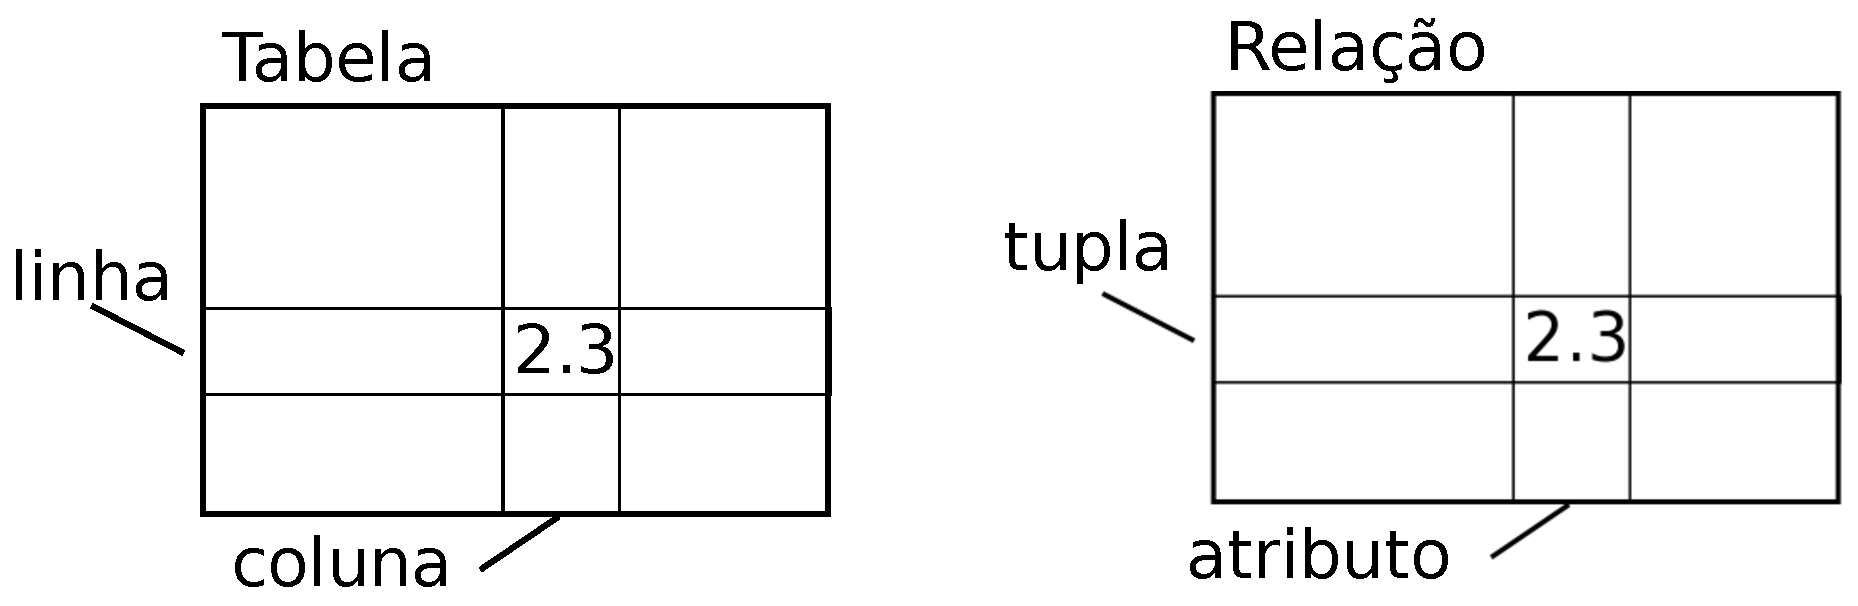
\includegraphics[height=1.50in]{figs2/relational.eps}}
\afterfig

%In technical descriptions of relational databases the concepts of 
%table, row, and column are more formally referred
%to as {\bf relation}, {\bf tuple}, and {\bf attribute}, respectively.
%We will use the less formal terms in this chapter.

Na descrição técnica de um banco de dados relacional o conceito de
tabela, linha e coluna são referências formais para {\bf relação},
{\bf tupla}, e {\bf atributo}, respectivamente.
Usaremos os termos menos formais neste capítulo.

%\section{SQLite manager Firefox add-on}
\section{Plugin do Firefox de Gerencia SQLite}
%While this chapter will focus on using Python to work with data 
%in SQLite database files, many operations can be done more
%conveniently using a Firefox add-on called the {\bf SQLite
%  Database Manager} which is freely available from:

O foco deste capítulo é o uso do Python para trabalhar com dados
com o SQLite, muitas operações podem ser feitas de forma mais
conveniente utilizando um {\it plugin} do Firefox, o {\bf SQLite
  Database Manager} que está disponível gratuitamente através do {\it link}:

\url{https://addons.mozilla.org/en-us/firefox/addon/sqlite-manager/}

%Using the browser you can easily create tables, insert data, edit data, 
%or run simple SQL queries on the data in the database.

Utilizando o navegador você pode facilmente criar tabelas, inserir, editar ou
executar consultas SQL nos dados da base de dados.

%In a sense, the database manager is similar to a text editor
%when working with text files.   When you want to do one or
%very few operations on a text file, you can just open it
%in a text editor and make the changes you want.   When you have 
%many changes that you need to do to a text file, often you 
%will write a simple Python program.  You will find the same 
%pattern when working with databases.  You will do simple
%operations in the database manager and more complex operations
%will be most conveniently done in Python.

De certa forma, o gerenciador de banco de dados é similar a um editor de texto
quando utilizado arquivos de texto. Quando você quer fazer uma ou mais
operações com um arquivo de texto, você pode simplesmente abrir o arquivo em
um editor de texto e fazer as alterações que desejar. Quando você tem que fazer
muitas alterações para fazer, normalmente você pode escrever um programa em
Python simples para executar esta tarefa. Você encontrará os mesmos padrões
quando for trabalhar com banco de dados. Você fará operações em um gerenciador
de banco de dados e as operações mais complexas serão mais convenientes se
forem feitas com Python.

%\section{Creating a database table}
\section{Criado uma tabela em um banco de dados}

%Databases require more defined structure than Python lists 
%or dictionaries\footnote{SQLite actually does allow some 
%flexibility in the type of data stored in a column,
%but we will keep our data types strict in this chapter
%so the concepts apply equally to other database systems 
%such as MySQL.}.

Bancos de dados precisam de estruturas mais bem definidas do quê listas ou
dicionários em Python\footnote{Atualmente o SQLite permite uma maior
  flexibilidade em relação aos tipos de dados que são armazenados em uma
  coluna, mas vamos manter os tipos de dados restritos neste capítulo, assim
  os mesmos conceitos aprendidos aqui podem ser aplicados a outros sistemas
  de banco de dados como MySQL.}.

%When we create a database {\bf table} we
%must tell the database in advance the names of each of the
%{\bf columns} in the table and the type of data which we are 
%planning to store in each {\bf column}.   When the database software
%knows the type of data in each column, it can choose the most 
%efficient way to store and look up the data based on the type of
%data.

Quando criamos uma {\bf tabela} em um banco de dados, precisamos informar ao
banco de dados previamente o nome de cada {\bf coluna} na tabela e o tipo de
dados que planejamos armazenar em cada {\bf coluna}. Quando o sistema de
banco de dados conhece o tipo de dado em cada coluna, ele pode definir a
forma mais eficiente de armazenar e consultar o dado baseado no tipo do dado.

%You can look at the various data types supported by SQLite
%at the following url:

Você pode visualizar os diversos tipos de dados que são suportados pelo SQLite
através do seguinte endereço:

\url{http://www.sqlite.org/datatypes.html}


%Defining structure for your data up front may seem inconvenient
%at the beginning, but the payoff is fast access to your data 
%even when the database contains a large amount of data.

Definir a estrutura dos seus tipos de dados pode parecer inconveniente no
começo, mas a recompensa é o acesso rápido aos dados mesmo quando o banco
de dados contém um grande número de informações.

%The code to create a database file and a table 
%named {\tt Tracks} with two columns in the 
%database is as follows:

O seguinte código cria um arquivo de banco de dados com uma tabela, chamada
{\tt Tracks} e com duas colunas:

\index{sqlite3 module}
\index{module!sqlite3}
\beforeverb
\begin{verbatim}
import sqlite3

conn = sqlite3.connect('music.sqlite3')
cur = conn.cursor()

cur.execute('DROP TABLE IF EXISTS Tracks ')
cur.execute('CREATE TABLE Tracks (title TEXT, plays INTEGER)')

conn.close()
\end{verbatim}
\afterverb
%
\index{connect function}
\index{function!connect}
\index{cursor function}
\index{function!cursor}
%The {\tt connect} operation makes a ``connection'' to the database 
%stored in the file {\tt music.sqlite3} in the current directory.   If
%the file does not exist, it will be created.  The reason this
%is called a ``connection'' is that sometimes the database is stored
%on a separate ``database server'' from the server on which we 
%are running our application.  In our simple examples 
%the database will just be a local file in the same directory
%as the Python code we are running.

A operação {\tt connect} cria uma ``conexão'' com o banco de dados armazenado
no arquivo {\tt music.sqlite3} no diretório corrente. Se o arquivo não
existir, este será criado. O motivo para isto ser chamado de ``conexão'' é
que algumas vezes o banco de dados está  em um ``servidor de banco de dados'' 
separado da aplicação propriamente dita. Em nossos exemplos o banco de dados
está armazenado localmente em um arquivo no mesmo diretório que o código
Python está sendo executado.


%A {\bf cursor} is like a file handle that we can use to perform
%operations on the data stored in the database.  Calling 
%{\tt cursor()} is very similar conceptually to calling
%{\tt open()} when dealing with text files.

Um {\bf cursos} é como um identificador de arquivo que podemos utilizar para
realizar operações sobre as informações armazenadas em um banco de dados. Ao
chamar a função {\tt cursor()}, conceitualmente, é similar ao chamar a função
{\tt open()} quando estamos trabalhando com arquivos de texto.

\beforefig
\centerline{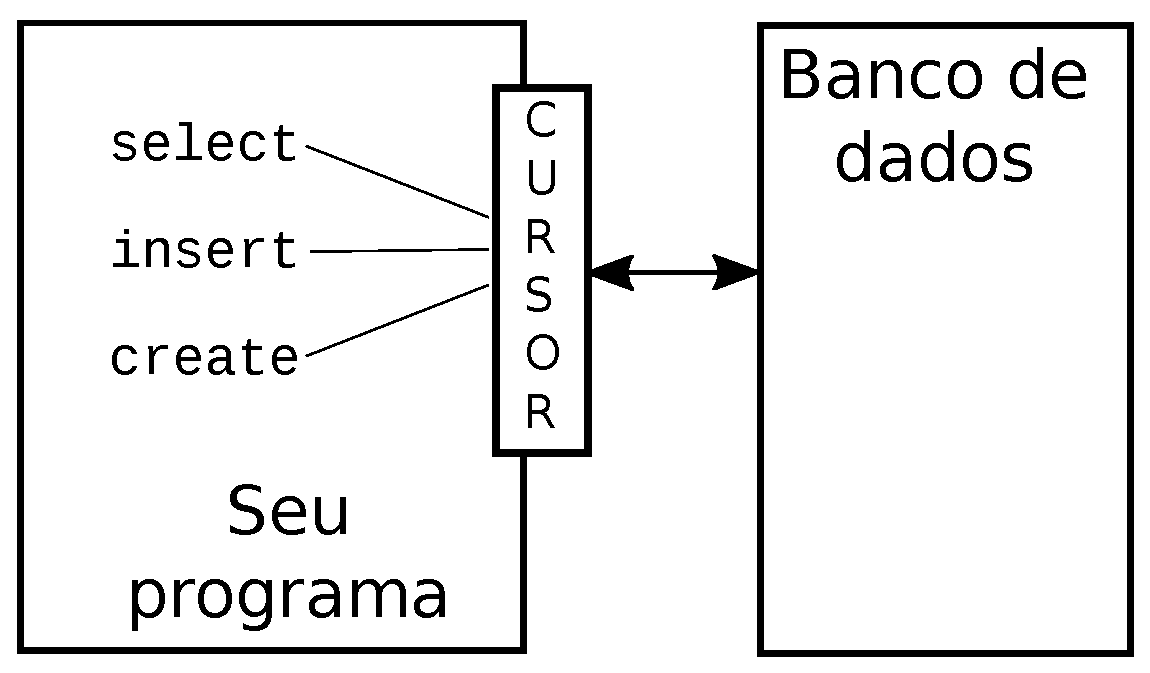
\includegraphics[height=1.50in]{figs2/cursor.eps}}
\afterfig

%Once we have the cursor, we can begin to execute 
%commands on the contents of the database using the {\tt execute()}
%method.

Uma vez que temos o cursos, podemos começar a executar comandos no conteúdo
armazenado no banco de dados utilizando o método {\tt execute()}.

%Database commands are expressed in a special language that has 
%been standardized across many different database vendors 
%to allow us to learn a single database language.   The database
%language is called {\bf Structured Query Language} or {\bf SQL}
%for short.

Os comandos de um banco de dados são expressos em uma linguagem especial que
foi padronizada por diferentes fornecedores de bancos de dados, que nos
permite aprender uma única linguagem. A linguagem dos bancos de dados é
chamada de {\bf Structured Query Language}\footnote{Em Português, pode ser
  chamada de Linguagem de Consulta Estruturada} ou referenciada pelo acrônimo
{\bf SQL}
\url{http://en.wikipedia.org/wiki/SQL}

%In our example, we are executing two SQL commands in our database.
%As a convention, we will show the SQL keywords in uppercase 
%and the parts of the command that we are adding (such as the
%table and column names) will be shown in lowercase.

Em nossos exemplos, estamos executando dois comandos SQL no banco de dados que
criamos. Convencionaremos que os comandos SQL serão mostrados em maiúsculas e
as partes que não são palavras reservadas do SQL (como os nomes das tabelas e
colunas) serão mostrados em minúsculas.

%The first SQL command removes the {\tt Tracks} table from the 
%database if it exists.  This pattern is simply to allow us to 
%run the same program to create the {\tt Tracks} table over 
%and over again without causing an error.  Note that the
%{\tt DROP TABLE} command deletes the table and all of its contents
%from the database (i.e., there is no ``undo'').

O primeiro comando SQL remove a tabela {\tt Tracks} do banco de dados se ela
existir. Este padrão nos permite executar o mesmo programa para criar a tabela
{\tt Tracks} repetidas vezes sem que cause erro. Perceba que o comando {\tt DROP
  TABLE} remove a tabela e todo o seu conteúdo do banco de dados (i.e., não é
possível desfazer esta operação)

\beforeverb
\begin{verbatim}
cur.execute('DROP TABLE IF EXISTS Tracks ')
\end{verbatim}
\afterverb
%
%The second command creates a table named
%{\tt Tracks} with a text column named {\tt title}
%and an integer column named {\tt plays}.
%
O segundo comando cria a tabela {\tt Tracks} com uma coluna chamada {\tt title}
com o tipo texto e uma coluna chamada {\tt plays} com o tipo inteiro.

\beforeverb
\begin{verbatim}
cur.execute('CREATE TABLE Tracks (title TEXT, plays INTEGER)')
\end{verbatim}
\afterverb
%
%Now that we have created a table named {\tt Tracks}, we can put some data
%into that table using the SQL {\tt INSERT} operation.   Again, we begin
%by making a connection to the database and obtaining the {\tt cursor}.
%We can then execute SQL commands using the cursor.
%
Agora que criamos a tabela {\tt Tracks}, podemos inserir algum dado dentro
dela utilizando a operação SQL {\tt INSERT}. Novamente, estamos
estabelecendo uma conexão com o banco de dados e obtendo o {\tt cursos}.
E então executamos o comando SQL utilizando o cursor.

%The SQL {\tt INSERT} command indicates which table we are using 
%and then defines a new row by listing the fields we want to 
%include {\tt (title, plays)} followed by the {\tt VALUES} we want
%placed in the new row.  We specify the values as question marks
%{\tt (?, ?)} to indicate that the actual values are passed in as a
%tuple {\tt ( 'My Way', 15 ) } as the second parameter to the
%{\tt execute()} call.

O comando SQL {\tt INSERT} indica qual tabela estamos utilizando, e em seguida, 
cria uma nova linha listando quais campos utilizaremos para incluir {\tt (title,
  plays)} seguido pelo comando {\tt VALUES} com os valores que desejamos
adicionar na nova linha. Especificamos os valores utilizando pontos de
interrogação {\tt (?, ?)} para indicar que os valores serão passados como
tuplas {\tt ( 'My Way', 15) } como um segundo parâmetro da chamada
{\tt execute()}.

\beforeverb
\begin{verbatim}
import sqlite3

conn = sqlite3.connect('music.sqlite3')
cur = conn.cursor()

cur.execute('INSERT INTO Tracks (title, plays) VALUES ( ?, ? )', 
    ( 'Thunderstruck', 20 ) )
cur.execute('INSERT INTO Tracks (title, plays) VALUES ( ?, ? )', 
    ( 'My Way', 15 ) )
conn.commit()

print 'Tracks:'
cur.execute('SELECT title, plays FROM Tracks')
for row in cur :
   print row

cur.execute('DELETE FROM Tracks WHERE plays < 100')
conn.commit()

cur.close()
\end{verbatim}
\afterverb
%
%First we {\tt INSERT} two rows into our table and use {\tt commit()} 
%to force the data to be written to the database file.

Primeiro nós adicionamos com {\tt INSERT} duas linha na nossa tabela e
usamos {\tt commit()} para forçar a escrita da informação no arquivo do banco
de dados.

\beforefig
\centerline{\includegraphics[height=1.00in]{figs2/tracks.eps}}
\afterfig

%Then we use the {\tt SELECT} command
%to retrieve the rows we just inserted from the table.  
%On the 
%{\tt SELECT} command, we indicate which columns we would like {\tt (title, plays)}
%and indicate which table we want to retrieve the data from.  After we 
%execute the {\tt SELECT} statement, the cursor is something we can loop through
%in a {\tt for} statement.   For efficiency,
%the cursor does not read all of the data from the
%database when we execute the {\tt SELECT} statement.  
%Instead, the data is read on demand
%as we loop through the rows in the {\tt for} statement.

Depois usamos o comando {\tt SELECT} para buscar a linha que acabamos de
inserir na tabela. Com o comando {\tt SELECT}, indicamos que coluna gostaríamos
{\tt (title, plays)} e de qual tabela queremos buscar a informação. Depois
de confirmar a executação do comando {\tt SELECT}, o cursor pode ser utilizado
como repetição através de um comando {\tt for}. Por questões de eficiência, o
cursor não lê toda a informação da base de dados quando executamos o comando
{\tt SELECT}. Ao invés disto, a informação é lida sob demanda enquanto
iteramos através da linha com o comando {\tt for}.

%The output of the program is as follows:

A saída do programa fica da seguinte forma:

\beforeverb
\begin{verbatim}
Tracks:
(u'Thunderstruck', 20)
(u'My Way', 15)
\end{verbatim}
\afterverb
%
\index{Unicode}
%Our {\tt for} loop finds two rows, and each row is a Python tuple with the
%first value as the {\tt title} and the second value as the number of {\tt plays}.
%Do not be concerned that the title strings are shown starting with 
%{\tt u'}.  This is an indication that the strings are {\bf Unicode} strings
%that are capable of storing non-Latin character sets.

A iteração do {\tt for} encontrou duas linhas, e cada linha é uma tupla em
Python com o primeiro valor como {\tt title} e o segundo como o número de
{\tt plays}. Não se preocupe com o fato de a {\it strings} são mostrados com
o caractere {\tt u'} no começo. Isto é uma indicação que a {\it string} estão
em {\bf Unicode}, o que indica que são capazes de armazenar um conjunto de
caractere não-Latin.

%At the very end of the program, we execute an SQL command to {\tt DELETE} 
%the rows we have just created so we can run the program over and over.
%The {\tt DELETE} command shows the use of a {\tt WHERE} clause that
%allows us to express a selection criterion so that we can ask the database
%to apply the command to only the rows that match the criterion.  In this example
%the criterion happens to apply to all the rows so we empty the table
%out so we can run the program repeatedly.  After the {\tt DELETE} is performed,
%we also call {\tt commit()} to force the data to be removed from the database.

No final do programa, executamos o comando SQL {\tt DELETE} para remover as
linhas que acabamos de criar, assim podemos executar o programa repetidas
vezes. O {\tt DELETE} pode ser utilizado com a condição {\tt WHERE} que permite
selecionar através de uma expressão o critério permitindo pesquisar no banco
de dados somente as linhas que correspondem com a expressão utilizada. Neste
exemplo a expressão construida se aplica em todas as linhas, para que possamos
executar o programa outras vezes. Depois de executar o {\tt DELETE} chamamos o
{\tt commit()} para forçar que o dado seja removido do banco de dados.

%\section{Structured Query Language summary}
\section{Resumo de Structured Query Language (SQL)}

%So far, we have been using the Structured Query Language in our Python
%examples and have covered many of the basics of the SQL commands.
%In this section, we look at the SQL language in particular
%and give an overview of SQL syntax.

Estamos utilizando SQL junto com os exemplos de Python e até agora cobrimos
muitos comandos SQL básicos. Nesta seção, vamos olhar a linguagem SQL com
mais atenção e apresentaremos uma visão geral da sintaxe do SQL.

%Since there are so many different database vendors, the Structured Query
%Language (SQL) was standardized so we could communicate in a portable
%manner to database systems from multiple vendors.

Existem diferentes fornecedores de bancos de dados, a linguagem SQL foi
padronizada, desta forma podemos nos comunicar de maneira portável entre os
diferentes sistemas de banco de dados dos diferentes fornecedores.

%A relational database is made up of tables, rows, and columns.  The columns
%generally have a type such as text, numeric, or date data.  When we create
%a table, we indicate the names and types of the columns:

Basicamente um banco de dados relacional é composto por tabelas, linhas e
colunas. As colunas geralmente possuem tipos, como textos, números ou
informação de data. Quando criamos uma tabela, indicamos os nomes e tipos das
colunas:

\beforeverb
\begin{verbatim}
CREATE TABLE Tracks (title TEXT, plays INTEGER)
\end{verbatim}
\afterverb
%
%To insert a row into a table, we use the SQL {\tt INSERT} command:
%
Para inserir uma linha em uma tabela, utilizamos o comando SQL {\tt INSERT}:

\beforeverb
\begin{verbatim}
INSERT INTO Tracks (title, plays) VALUES ('My Way', 15)
\end{verbatim}
\afterverb
%
%The {\tt INSERT} statement specifies the table name, then a list of
%the fields/columns that you would like to set in the new row, and then 
%the keyword {\tt VALUES} and a list of corresponding values 
%for each of the fields.
%
A declaração do {\tt INSERT} especifica o nome da tabela, e então, uma lista
dos campos/colunas que gostaríamos de definir na nova linha, e por fim,
através do campo {\tt VALUES} passamos uma lista de valores correspondentes a
cada campo.

%The SQL {\tt SELECT} command is used to retrieve rows and columns from a database.
%The {\tt SELECT} statement lets you specify which columns you would
%like to retrieve as well as a {\tt WHERE} clause to select which 
%rows you would like to see.  It also allows an optional 
%{\tt ORDER BY} clause to control the sorting of the returned rows.

O comando {\tt SELECT} é utilizado para buscar as linhas e colunas de um banco
de dados. A declaração do {\tt SELECT} permite que você especifique qual coluna
gostaria de buscar, bem como utilizando a condição do {\tt WHERE}, permite
selecionar qual linha gostaríamos de visualizar. Isto também possibilita o uso
de uma condição opcional, {\tt ORDER BY}, para ordenar as linhas retornadas.

\beforeverb
\begin{verbatim}
SELECT * FROM Tracks WHERE title = 'My Way'
\end{verbatim}
\afterverb
%
%Using \verb"*" indicates that you want the database to return all of 
%the columns for each row that matches the {\tt WHERE} clause.

O uso do \verb"*" indica que o banco de dados deve retornar todas as colunas
para cada linha que casa com a condição {\tt WHERE}.

%Note, unlike in Python, in a SQL {\tt WHERE} clause 
%we use a single equal sign 
%to indicate a test for equality rather than a double equal sign.
%Other logical operations allowed in a {\tt WHERE} clause include

Atenção, diferente de Python, a condição {\tt WHERE}, em SQL, utiliza o sinal
de igual simples (\verb"="), para indicar uma condição de igualdade, ao invés de
um sinal duplo (\verb"==")
\verb"<",
\verb">",
\verb"<=",
\verb">=",
\verb"!=",
%as well as {\tt AND} and {\tt OR} and parentheses
%to build your logical expressions.

assim como é possível utilizar as condições {\tt AND} e {\tt OR} e parênteses
para construir expressões lógicas.

%You can request that the returned rows be sorted by one of 
%the fields as follows:

Você pode pedir que as linhas retornadas sejam ordenadas por um dos campos
como apresentados no exemplo a seguir:
\beforeverb
\begin{verbatim}
SELECT title,plays FROM Tracks ORDER BY title
\end{verbatim}
\afterverb
%
%To remove a row, you need a {\tt WHERE} clause on an SQL {\tt DELETE}
%statement.  The {\tt WHERE} clause determines which rows are to be deleted:
%
Para remover uma linha, é preciso combinar a condição {\tt WHERE} com a
condição {\tt DELETE}. O {\tt WHERE} irá determinar quais linhas serão
removidas:

\beforeverb
\begin{verbatim}
DELETE FROM Tracks WHERE title = 'My Way'
\end{verbatim}
\afterverb
%
%It is possible to {\tt UPDATE} a column or columns within one or more rows
%in a table using the SQL {\tt UPDATE} statement as follows:
%
É possível alterar/atualizar uma ou mais colunas e suas linhas de uma tabela
utilizando a condição SQL {\tt UPDATE}, da seguinte forma:

\beforeverb
\begin{verbatim}
UPDATE Tracks SET plays = 16 WHERE title = 'My Way'
\end{verbatim}
\afterverb
%
%The {\tt UPDATE} statement specifies a table and 
%then a list of fields and values to change after the {\tt SET} 
%keyword and then an optional {\tt WHERE} clause to select
%the rows that are to be updated.  A single {\tt UPDATE} statement
%will change all of the rows that match the {\tt WHERE} clause.  If 
%a {\tt WHERE} clause is not specified, it performs the {\tt UPDATE}
%on all of the rows in the table.
%
A condição {\tt UPDATE} especifica uma tabela e depois uma lista de campos e
valores que serão alterados após o comando {\tt SET}, e utilizando uma condição
{\tt WHERE}, opctional, é possível selecionar as linhas que serão atualizadas.
Uma condição {\tt UPDATE} irá mudar todas as linhas que casam com a condição
{\tt WHERE}. Se a condição {\tt WHERE} não for especificada, o {\tt UPDATE}
será aplicado em todas as linhas da tabela.

%These four basic SQL commands (INSERT, SELECT, UPDATE, and DELETE) allow 
%the four basic operations needed to create and maintain data.

Os quatros comandos básicos de SQL (INSERT, SELECT, UPDTE e DELETE) permitem
as quatro operações básicas necessárias para criação e manutenção das
informações em um banco de dados.

%\section{Spidering Twitter using a database}
\section{Rastreando o Twitter utilizando um banco de dados}

%In this section, we will create a simple spidering program that will 
%go through Twitter accounts and build a database of them.
%\emph{Note: Be very careful when running this program.  You do not
%want to pull too much data or run the program for too long and
%end up having your Twitter access shut off.}

Nesta seção criaremos um programa simples para rastreamento que navegará
através de contas de usuários do Twitter e construirá um banco de dados
destas referentes as estes usuários.
\emph{Nota: Tenha muito cuidado ao executar este programa. Você não irá querer
  extrair muitas informações ou executar o programa por muito tempo e acabar
  tendo sua conta do Twitter bloqueada.}

%One of the problems of any kind of spidering program is that it 
%needs to be able to be stopped and restarted many times and 
%you do not want to lose the data that you have retrieved so far.
%You don't want to always restart your data retrieval at the
%very beginning so we want to store data as we retrieve it so our
%program can start back up and pick up where it left off.

Um dos problemas, em qualquer tipo de programas de rastreamento, é que precisa
ser capaz de ser interrompido e reiniciado muitas vezes e você não quer perder
informações que você já tenha recuperado até agora. Não quer sempre reiniciar
a recuperação dos dados desde o começo, então armazenamos as informações tão
logo seja recuperada, assim o programa poderá reiniciar a busca do ponto onde
parou.


%We will start by retrieving one person's Twitter friends and their
%statuses, looping through the list of friends, and adding each 
%of the friends to a database to be retrieved in the future.  After
%we process one person's Twitter friends, we check in our database
%and retrieve one of the friends of the friend.  We do this over and
%over, picking an ``unvisited'' person, retrieving their friend list,
%and adding friends we have not seen to our list for a future visit.

Vamos começar recuperando os amigos de uma pessoa no Twitter e seus status,
iterando na lista de amigos, e adicionando cada um ao banco de dados para
que possa ser recuperado no futuro. Depois de listar os amigos de uma pessoa,
verificamos na nossa base de dados e coletamos os amigos de um dos amigos da
primeira pessoa. Vamos fazendo isto repetidas vezes, escolhendo umas das
pessoas ``não visitadas'', recuperando sua lista de amigos, e
adicionando amigos que não tenhamos visto anteriormente a nossa lista, para
visitar futuramente.

%We also track how many times we have seen a particular friend in the
%database to get some sense of their ``popularity''.

Também rastrearemos quantas vezes vimos um amigo em particular na nossa base
para ter uma ideia da sua ``popularidade''.

%By storing our list of known accounts and whether 
%we have retrieved the account or not, 
%and how popular the account is in a database on the disk
%of the computer, we can stop and
%restart our program as many times as we like.

Armazenando nossa lista de contas conhecidas, no banco de dados no disco do
nosso computador, e se já recuperamos a conta ou não, e quanto esta conta é
popular, podemos parar e recomeçar nosso programa quantas vezes quisermos.

% TODO: Add a reference to the right spot
%This program is a bit complex. It is based on the code 
%from the exercise earlier in the book that uses
%the Twitter API.

% TODO: Adicionar a referência do código para o lugar certo.
Este programa é um pouco complexo. É baseado em um exercício apresentado
anteriormente neste livro, que utiliza a API do Twitter

%Here is the source code for our Twitter spidering application:

O seguinte código apresenta o programa que realiza o rastreamento no Twitter:

\beforeverb
\begin{verbatim}
import urllib
import twurl
import json
import sqlite3

TWITTER_URL = 'https://api.twitter.com/1.1/friends/list.json'

conn = sqlite3.connect('spider.sqlite3')
cur = conn.cursor()

cur.execute('''
CREATE TABLE IF NOT EXISTS Twitter 
(name TEXT, retrieved INTEGER, friends INTEGER)''')

while True:
    acct = raw_input('Enter a Twitter account, or quit: ')
    if ( acct == 'quit' ) : break
    if ( len(acct) < 1 ) :
        cur.execute('SELECT name FROM Twitter WHERE retrieved = 0 LIMIT 1')
        try:
            acct = cur.fetchone()[0]
        except:
            print 'No unretrieved Twitter accounts found'
            continue

    url = twurl.augment(TWITTER_URL, 
               {'screen_name': acct, 'count': '20'} )
    print 'Retrieving', url
    connection = urllib.urlopen(url)
    data = connection.read()
    headers = connection.info().dict
    # print 'Remaining', headers['x-rate-limit-remaining']
    js = json.loads(data)
    # print json.dumps(js, indent=4)

    cur.execute('UPDATE Twitter SET retrieved=1 WHERE name = ?', (acct, ) )

    countnew = 0
    countold = 0
    for u in js['users'] :
        friend = u['screen_name']
        print friend
        cur.execute('SELECT friends FROM Twitter WHERE name = ? LIMIT 1', 
            (friend, ) )
        try:
            count = cur.fetchone()[0]
            cur.execute('UPDATE Twitter SET friends = ? WHERE name = ?', 
                (count+1, friend) )
            countold = countold + 1
        except:
            cur.execute('''INSERT INTO Twitter (name, retrieved, friends) 
                VALUES ( ?, 0, 1 )''', ( friend, ) )
            countnew = countnew + 1
    print 'New accounts=',countnew,' revisited=',countold
    conn.commit()

cur.close()
\end{verbatim}
\afterverb
%
%Our database is stored in the file {\tt spider.sqlite3} and it has one 
%table named {\tt Twitter}.  Each row in the {\tt Twitter} table
%has a column for the account name, whether we have retrieved the friends
%of this account, and how many times this account has been ``friended''.

%
Nossa base de dados está armazenada no arquivo {\tt spider.sqlite3} e possui
uma tabela chamada {\tt Twitter}. Cada linha na tabela {\tt Twitter} tem uma
coluna para o nome da conta, se recuperamos os amigos desta conta, e quantas
vezes esta conta foi ``seguido''.

%In the main loop of the program, we prompt the user for a Twitter
%account name or ``quit'' to exit the program.  
%If the user enters a Twitter account, we retrieve the 
%list of friends and statuses
%for that user and add each friend to the database if 
%not already in the database.  If the friend is already in the list, 
%we add 1 to the {\tt friends} field in the row in the database.

Na repetição principal do programa, perguntamos ao usuário uma conta de Twitter
ou ``quit'' para sair do programa. Se o usuário informar um usuário do Twitter,
o programa começa a recuperar a lista de amigos e os status para aquele
usuário e adiciona cada amigo na base de dados se não possuir. Se o amigo já
está na lista, nós adicionamos ``1'' no campo {\tt friends} da base de dados.


%If the user presses enter, we look in the database for the next 
%Twitter account that we have not yet retrieved, retrieve the
%friends and statuses for that account, add them to the database 
%or update them, and increase their {\tt friends} count.

Se o usuário pressionar {\tt enter}, pesquisamos na base a próxima conta que
não rastreamos ainda, e então rastreamos os amigos e status com aquela conta
e adicionamos na base de dados ou atualizamos, incrementando seu contador de
{\tt friends}.

%Once we retrieve the list of friends and statuses, we loop 
%through all of the {\tt user} items in the returned JSON
%and retrieve the \verb"screen_name" for each user.  Then we use
%the {\tt SELECT} statement to see if we already have stored this
%particular \verb"screen_name" in the database and retrieve the
%friend count ({\tt friends}) if the record exists.

Uma vez que rastreamos a lista de amigos e status, iteramos entre todas os
ítens {\tt user} retornados no JSON e rastreamos o  \verb"screen_name" para
cada usuário. Então utilizamos a declaração {\tt SELECT} para ver se já
armazenamos este \verb"screen_name" em particular na base e recuperamos o
contador de amigos ({\tt friends}), se este registro existir.

\beforeverb
\begin{verbatim}
    countnew = 0
    countold = 0
    for u in js['users'] :
        friend = u['screen_name']
        print friend
        cur.execute('SELECT friends FROM Twitter WHERE name = ? LIMIT 1', 
            (friend, ) )
        try:
            count = cur.fetchone()[0]
            cur.execute('UPDATE Twitter SET friends = ? WHERE name = ?', 
                (count+1, friend) )
            countold = countold + 1
        except:
            cur.execute('''INSERT INTO Twitter (name, retrieved, friends) 
                VALUES ( ?, 0, 1 )''', ( friend, ) )
            countnew = countnew + 1
    print 'New accounts=',countnew,' revisited=',countold
    conn.commit()
\end{verbatim}
\afterverb
%
%Once the cursor executes the {\tt SELECT} statement, 
%we must retrieve the rows.  We could do this with a {\tt for} 
%statement, but since we are only retrieving
%one row ({\tt LIMIT 1}), we can use the {\tt fetchone()} method to fetch the
%first (and only) row that is the result of the {\tt SELECT} operation.  
%Since {\tt fetchone()} returns the row as a {\bf tuple} (even though there is only
%one field), we take the first value from the tuple using {\tt [0]} to get the 
%current friend count into the variable {\tt count}.  

%
Uma vez que o cursor tenha executado o {\tt SELECT}, nós devemos recuperar as
linhas. Podemos fazer isto com uma declaração de {\tt for}, mas uma vez que
estamos recuperando uma linha ({\tt LIMIT 1}), podemos utilizar o método
{\tt fetchone()} para buscar a primeira (e única) linha que é o resultado da
operação {\tt SELECT}. Sendo o retorno {\tt fetchone()} uma linha como uma
{\bf tupla} (ainda que haja somente um campo), pegamos o primeiro valor da
tupla utilizando índice {\tt [0]} para pegar o contador de amigos atual dentro
da variável {\tt count}.

%If this retrieval is successful, we use the SQL {\tt UPDATE} statement with a 
%{\tt WHERE} clause to add 1 to the {\tt friends} column for the row that 
%matches the friend's account.  Notice that there are two placeholders (i.e.,
%question marks) in the SQL, and the second parameter to the {\tt execute()} is
%a two-element tuple that holds the values to be substituted into the SQL
%in place of the question marks.

Se a busca for bem sucedida, utilizamos a declação {\tt UPDATE} com a clausula 
{\tt WHERE} para adicionar 1 na coluna {\tt friends} para a linha que
corresponde com a conta do amigo. Note que existem dois espaços reservados
(i.e., pontos de interrogações) no SQL, e o segundo parâmetro para o
{\tt execute()} é uma tupla que armazena o valor para substituir no SQL no
lugar dos pontos de interrogações.

%If the code in the {\tt try} block fails, it is probably because no record
%matched the {\tt WHERE name = ?} clause on the SELECT statement.  So in the
%{\tt except} block, we use the SQL {\tt INSERT} statement to add the friend's
%\verb"screen_name" to the table with an indication that we have not yet 
%retrieved the \verb"screen_name" and set the friend count to zero.

Se o bloco {\tt try} falhar, é provavelmente por que nenhum resultado
corresponde a clausula em {\tt WHERE name = ?} do SELECT. Então no block
{\tt except}, utilizamos a declaração {\tt INSERT} para adicionar o
\verb"screen_name" do amigo a tabela com a indicação que ainda não rastreamos
o \verb"screen_name" e setamos o contador de amigos com 0 (zero).

%So the first time the program runs and we enter a Twitter account, the program
%runs as follows:

Assim, a primeira vez que o programa é executado e informamos uma conta do
Twitter, a saída do programa é a seguinte:

\beforeverb
\begin{verbatim}
Enter a Twitter account, or quit: drchuck
Retrieving http://api.twitter.com/1.1/friends ...
New accounts= 20  revisited= 0
Enter a Twitter account, or quit: quit
\end{verbatim}
\afterverb
%
%Since this is the first time we have run the program, the database
%is empty and we create the database in the file {\tt spider.sqlite3} and
%add a table named {\tt Twitter} to the database.  Then we retrieve
%some friends and add them all to the database since the database is
%empty.

Como esta é a primeira vez que executamos o programa, o banco de dados está
vazio e criamos o banco no arquivo {\tt spider.sqlite3}, adicionamos a tabela
chamada {\tt Twitter} na base de dados. Então nós rastreamos alguns amigos e
os adicionamos a base, uma vez que ela está vazia.

%At this point, we might want to write a simple database dumper
%to take a look at what is in our {\tt spider.sqlite3} file:

Neste ponto podemos escrever um {\it dumper} simples para olhar o que está no
nosso arquivo {\tt spider.sqlite3}:

\beforeverb
\begin{verbatim}
import sqlite3

conn = sqlite3.connect('spider.sqlite3')
cur = conn.cursor()
cur.execute('SELECT * FROM Twitter')
count = 0
for row in cur :
   print row
   count = count + 1
print count, 'rows.'
cur.close()
\end{verbatim}
\afterverb
%
%This program simply opens the database and selects all of the 
%columns of all of the rows in the table {\tt Twitter}, then 
%loops through the rows and prints out each row.

%
Este programa abre o banco de dados e seleciona todas as colunas de todas as
linhas na tabela {\tt Twitter}, depois itera em cada linha e imprime o valor
dentro de cada uma.

%If we run this program after the first execution of our Twitter
%spider above, its output will be as follows:

Se executarmos este programa depois da primeira execução do nosso rastreador
{\it spider} do Twitter, sua saída será como a seguinte:

\beforeverb
\begin{verbatim}
(u'opencontent', 0, 1)
(u'lhawthorn', 0, 1)
(u'steve_coppin', 0, 1)
(u'davidkocher', 0, 1)
(u'hrheingold', 0, 1)
...
20 rows.
\end{verbatim}
\afterverb
%
%We see one row for each \verb"screen_name", that we 
%have not retrieved the data for that \verb"screen_name", and 
%everyone in the database has one friend.

%
Veremos uma linha para cada \verb"screen_name", que não tenhamos recuperado
o dado daquele \verb"screen_name", e todos tem um amigo.

%Now our database reflects the retrieval of the friends of 
%our first Twitter account ({\bf drchuck}).  We can run the program
%again and tell it to retrieve the friends of the next 
%``unprocessed'' account by simply pressing enter instead of
%a Twitter account as follows:

Agora nosso banco de dados reflete quais amigos estão relacionados com a nossa
primeira conta do Twitter ({\bf drchuck}) utilizada para rastreamento. Podemos
executar o programa novamente e mandar rastrear a próxima conta
``não processada'' e recuperar os amigos, simplemente pressionando {\tt enter}
ao invés de informar uma conta do Twitter, conforme o exemplo a seguir:


\beforeverb
\begin{verbatim}
Enter a Twitter account, or quit: 
Retrieving http://api.twitter.com/1.1/friends ...
New accounts= 18  revisited= 2
Enter a Twitter account, or quit: 
Retrieving http://api.twitter.com/1.1/friends ...
New accounts= 17  revisited= 3
Enter a Twitter account, or quit: quit
\end{verbatim}
\afterverb
%
%Since we pressed enter (i.e., we did not specify a Twitter account),
%the following code is executed:

%
Uma vez que pressionamos {\tt enter} (i.e., não especificamos uma conta do
Twitter), o seguinte código é executado:

\beforeverb
\begin{verbatim}
    if ( len(acct) < 1 ) :
        cur.execute('SELECT name FROM Twitter WHERE retrieved = 0 LIMIT 1')
        try:
            acct = cur.fetchone()[0]
        except:
            print 'No unretrieved twitter accounts found'
            continue
\end{verbatim}
\afterverb
%
%We use the SQL {\tt SELECT} statement to retrieve the name of the first 
%({\tt LIMIT 1}) user who still has their ``have we retrieved this user''
%value set to zero.  We also use the {\tt fetchone()[0]} pattern within 
%a try/except block to either extract a \verb"screen_name" from the retrieved
%data or put out an error message and loop back up.

%
Utilizamos a declaração SQL {\tt SELECT} para recuperar o nome do primeiro
({\tt LIMIT 1}) usuário que ainda tem seu ``recuperamos este usuário'' com o
valor setado em zero. Também utilizamos o padrão {\tt fetchone()[0]} dentro de
um bloco try/except para extrair também um \verb"screen_name" do dado
recuperado ou apresentamos uma mensagem de erro e iteramos novamente.

%If we successfully retrieved an unprocessed \verb"screen_name", we retrieve
%their data as follows:

Se tivermos sucesso ao recuperar um \verb"screen_name" não processado, vamos
extrair seus dados da seguinte maneira:

\beforeverb
\begin{verbatim}
    url = twurl.augment(TWITTER_URL, {'screen_name': acct, 'count': '20'} )
    print 'Retrieving', url
    connection = urllib.urlopen(url)
    data = connection.read()
    js = json.loads(data)

    cur.execute('UPDATE Twitter SET retrieved=1 WHERE name = ?', (acct, ) )
\end{verbatim}
\afterverb
%
%Once we retrieve the data successfully, we use the {\tt UPDATE} statement 
%to set the {\tt retrieved} column to 1 to indicate that we have completed 
%the retrieval of the friends of this account.  This keeps us from retrieving
%the same data over and over and keeps us progressing forward through the network
%of Twitter friends.
%
Ao recuperar os dados com sucesso, utilizaremos a declaração {\tt UPDATE} para
setar a coluna {\tt retrieved} para 1 para indicar que completamos a extração
dos amigos relacionados com esta conta. Isto no permite recuperar o mesmo dado
diversas vezes e nos permite prosseguir através da lista de amigos no Twitter. 

%If we run the friend program and press enter twice to retrieve the next 
%unvisited friend's friends,
%then run the dumping program, it will give us the following output:

Se executarmos o programa novamente, e pressionarmos {\tt enter} duas vezes
seguidas para recuperar os próximos amigos do amigo e depois executarmos o
programa de {\it dumping}, ele nos mostrará a seguinte saída:

\beforeverb
\begin{verbatim}
(u'opencontent', 1, 1)
(u'lhawthorn', 1, 1)
(u'steve_coppin', 0, 1)
(u'davidkocher', 0, 1)
(u'hrheingold', 0, 1)
...
(u'cnxorg', 0, 2)
(u'knoop', 0, 1)
(u'kthanos', 0, 2)
(u'LectureTools', 0, 1)
...
55 rows.
\end{verbatim}
\afterverb
%
%We can see that we have properly recorded that we have visited 
%{\tt lhawthorn} and {\tt opencontent}.  Also the accounts 
%{\tt cnxorg} and {\tt kthanos} already have two followers.
%Since we now have retrieved the friends of three people
%({\tt drchuck}, {\tt opencontent}, and {\tt lhawthorn}) our table has 55 rows 
%of friends to retrieve.

Podemos ver que gravamos de forma apropriada que visitamos os usuários
{\tt lhawthorn} e {\tt opencontent}. E que as contas {\tt cnxorg} e
{\tt kthanos} já tem dois seguidores. Desde que tenhamos recuperado os amigos
de três pessoas ({\tt drchuck}, {\tt opencontent}, e {\tt lhawthorn}) nossa
tabela tem agora 55 linhas de amigos recuperados.

%Each time we run the program and press enter it will pick the next 
%unvisited account (e.g., the next account will be \verb"steve_coppin"),
%retrieve their friends, mark them as retrieved, and for each of the 
%friends of \verb"steve_coppin" either add them to the end of the 
%database or update their friend count if they are already in the
%database.

Cada vez que executamos o programa e pressionamos {\tt enter} ele pegará a
próxima conta não visitada (e.g., a próxima conta será \verb"steve_coppin"),
recuperar seus amigos, marcá-los como recuperados, e para cada um dos amigos
de \verb"steve_coppin" também adicionaremos eles para no fim da base de dados 
e atualizaremos seus amigos que já estiverem na base de dados.

%Since the program's data is all stored on disk in a database, 
%the spidering activity can be suspended and resumed as many times as you 
%like with no loss of data.

Assim que os dados do programa estejam armazenados no disco em um banco de
dados o rastreamento pode ser suspenso e reiniciado tantas vezes quando
quiser sem a perda de informações.

%\section{Basic data modeling}
\section{Modelagem de dados básica}

%The real power of a relational database is when we create multiple tables
%and make links between those tables.   The act of deciding how to break
%up your application data into multiple tables and establishing the
%relationships between the tables is called {\bf data modeling}.  The
%design document that shows the tables and their relationships 
%is called a {\bf data model}.

O verdadeiro poder de um banco de dados relacional é quando criamos múltiplas
tabelas e criamos ligações entre elas. Decidir como dividir os dados da sua
aplicação em diferentes tabelas e estabelecer a relação entre estas tabelas é
o que chamamos de {\bf modelagem de dados}. O documento que mostra a estrutura 
das tabelas e suas relações é chamado de {\bf modelo de dados}.

%Data modeling is a relatively sophisticated skill and we will only introduce
%the most basic concepts of relational data modeling in this section.  For more
%detail on data modeling you can start with:

Modelagem de dados é uma habilidade relativamente sofisticada e nesta seção
nós iremos somente introduzir os conceitos mais básicos da modelagem de dados
relacionais. Para maiores detalhes sobre modelagem de dados você pode começar
com:

\url{http://en.wikipedia.org/wiki/Relational_model}

%Let's say for our Twitter spider application, instead of just
%counting a person's friends, we wanted to keep a list of 
%all of the incoming relationships so we could find a list of 
%everyone who is following a particular account.

Digamos que para a nossa aplicação de rastreamento do Twitter, ao invés de
só contar os amigos das pessoas, nós queiramos manter uma lista de todas as
relações de entrada, então poderemos encontrar uma lista de todos que seguem
uma pessoa em particular.

%Since everyone will potentially have many accounts that follow
%them, we cannot simply add a single column to our {\tt Twitter} table. 
%So we create a new table that keeps track of pairs of friends.
%The following is a simple way of making such a table:

Já que todos, potencialmente, terão tantas contas que o sigam, nós não podemos
simplesmente adicionar uma coluna para nossa tabela {\tt Twitter}. Então
criamos uma nova tabela que mantém o controle dos pares de amigos. A seguir
temos uma forma simples de criar tal tabela:

\beforeverb
\begin{verbatim}
CREATE TABLE Pals (from_friend TEXT, to_friend TEXT)
\end{verbatim}
\afterverb
%
%Each time we encounter a person who {\tt drchuck} is following, we
%would insert a row of the form:
%
Toda vez que encontrarmos uma pessoa que {\tt drchuck} está seguindo, nós
iremos inserir uma linha da seguinte forma:

\beforeverb
\begin{verbatim}
INSERT INTO Pals (from_friend,to_friend) VALUES ('drchuck', 'lhawthorn')
\end{verbatim}
\afterverb
%
%As we are processing the 20 friends from the {\tt drchuck}
%Twitter feed, we will insert 20 records with ``drchuck''
%as the first parameter so we will end up duplicating the 
%string many times in the database.
%
Como estamos processando 20 amigos da conta do {\it Twitter} do {\tt drchuck},
inserimor 20 registros com ``drchuck'' como primeiro parâmetro e assim
acaberemos duplicando a {\it string} muitas vezes no banco de dados.

%This duplication of string data violates one of the best practices 
%for {\bf database normalization} which basically states that
%we should never put the same string data in the database more than once.  
%If we need the data more than once, we create a 
%numeric {\bf key} for the data and reference the actual data 
%using this key.

Esta duplicação de dados viola uma das melhores práticas da {\bf normatização
  de banco de dados} que basicamente afirma que nunca devemos colocar o mesmo
dado mais de uma vez em um banco de dados. Se precisarmos inserir um dado mais
de uma vez, criamos uma referência numérica {\bf key} (chave) para o dado, e
utilizamos a chave para referenciar o dado.

%In practical terms, a string takes up a lot more 
%space than an integer on the disk
%and in the memory of our computer, and takes more processor time
%to compare and sort.  If we only have a few hundred entries, 
%the storage and processor time hardly matters.  But if we have 
%a million people in our database and a possibility of 100 million
%friend links, it is important to be able to scan data as quickly
%as possible.

Na prática, uma {\it string} ocupa muito mais espaço do que um inteiro, no
disco e na memória do nosso computador, e leva mais tempo do processor para
comparar e ordenar. Se tivermos somente algumas centenas de entradas, a base
de dados e o tempo de processamento dificilmente importarão. Mas se tivermos
um milhão de pessoas na nossa base de dados e uma possibilidade de 100 milhões
de conexões de amigos, é importante permitir examinar os dados o mais rápido
possível.

%We will store our Twitter accounts in a table named {\tt People}
%instead of the {\tt Twitter} table used in the previous example.
%The {\tt People} table has an additional column 
%to store the numeric key associated with the 
%row for this Twitter user.   
%SQLite has a feature that automatically adds the key value
%for any row we insert into a table using a special type of 
%data column ({\tt INTEGER PRIMARY KEY}).

Nós armazenaremos nossas contas do Twitter em uma tabela chamada {\tt People}
ao invés de utilizar a tabela {\tt Twitter} utilizada no exemplo anterior. A
tabela {\tt People} tem uma coluna adicional para armazenar uma chave associada
a linha para este usuário.

%We can create the {\tt People} table with this additional 
%{\tt id} column as follows:

Podemos criar a tabela {\tt People} com esta coluna {\tt id} adicional com o
seguinte comando:

\beforeverb
\begin{verbatim}
CREATE TABLE People 
    (id INTEGER PRIMARY KEY, name TEXT UNIQUE, retrieved INTEGER)
\end{verbatim}
\afterverb
%
%Notice that we are no longer maintaining a friend count in each row
%of the {\tt People} table.
%When we select {\tt INTEGER PRIMARY KEY} as the type of our {\tt id} column,
%we are indicating that we would like SQLite to manage this column and 
%assign a unique numeric key to each row we insert automatically.
%We also add the keyword {\tt UNIQUE} to indicate that we will not 
%allow SQLite to insert two rows with the same value for {\tt name}.
%
Perceba que nós não estamos mais mantendo uma conta de amigo em cada linha da
tabela {\tt People}. Quando selecionamos {\tt INTEGER PRIMARY KEY} como o tipo
da nossa coluna {\tt id}, estamos indicando que gostaríamos que o SQLite
gerencie esta coluna e defina uma chave numérica única automagicamente para
cada linha que inserirmos. Também adicionamos uma palavra-chave {\tt UNIQUE}
para indicar que não permitiremos ao SQLite inserir duas linhas com o mesmo
valor para {\tt name}.

%Now instead of creating the table {\tt Pals} above, we create
%a table called {\tt Follows} with two integer columns
%\verb"from_id" and \verb"to_id" and a constraint on the table that
%the \emph{combination} of \verb"from_id" and \verb"to_id" must be unique 
%in this table (i.e., we cannot insert duplicate rows) in our database.

Agora, ao invés de criar a tabela {\tt Pals} acima, criaremos uma tabela
chamada {\tt Follows} com duas colunas com o tipo inteiro \verb"from_id" e
\verb"to_id" e associaremos na tabela onde a \emph{combinação} de
\verb"from_id" e \verb"to_id" devem ser únicos nesta tabela (i.e., não podemos
inserir linhas duplicadas) na nossa base de dados.

\beforeverb
\begin{verbatim}
CREATE TABLE Follows 
    (from_id INTEGER, to_id INTEGER, UNIQUE(from_id, to_id) )
\end{verbatim}
\afterverb
%
%When we add {\tt UNIQUE} clauses to our tables, we are communicating a set
%of rules that we are asking the database to enforce when we attempt to insert
%records.   We are creating these rules as a convenience in our programs, as we
%will see in a moment.  The rules both keep us from making mistakes and make
%it simpler to write some of our code.

Quando adicionamos a condição {\tt UNIQUE} a nossa tabela, estamos definindo
um conjunto de regras e pedindo a base de dados para cumprir estas regras
quando tentarmos inserir algum registro. Estamos criando estas regras como uma
conveniencia no nosso programa, como veremos a seguir. As regras nos impede de
cometer enganos e facilita na escrita dos nossos códigos.

%In essence, in creating this {\tt Follows} table, we are modelling a 
%``relationship'' where one person ``follows'' someone else
%and representing it with a pair of numbers indicating that (a) the people are
%connected and (b) the direction of the relationship.

Em essencia, criando a tabela {\tt Follows}, estamos modelando uma ``relação''
onde uma pessoa ``segue'' outro alguém e representamos isto com um par de
números indicando que (a) as pessoas estão conectadas e (b) a direção do
relacionamento.

\beforefig
\centerline{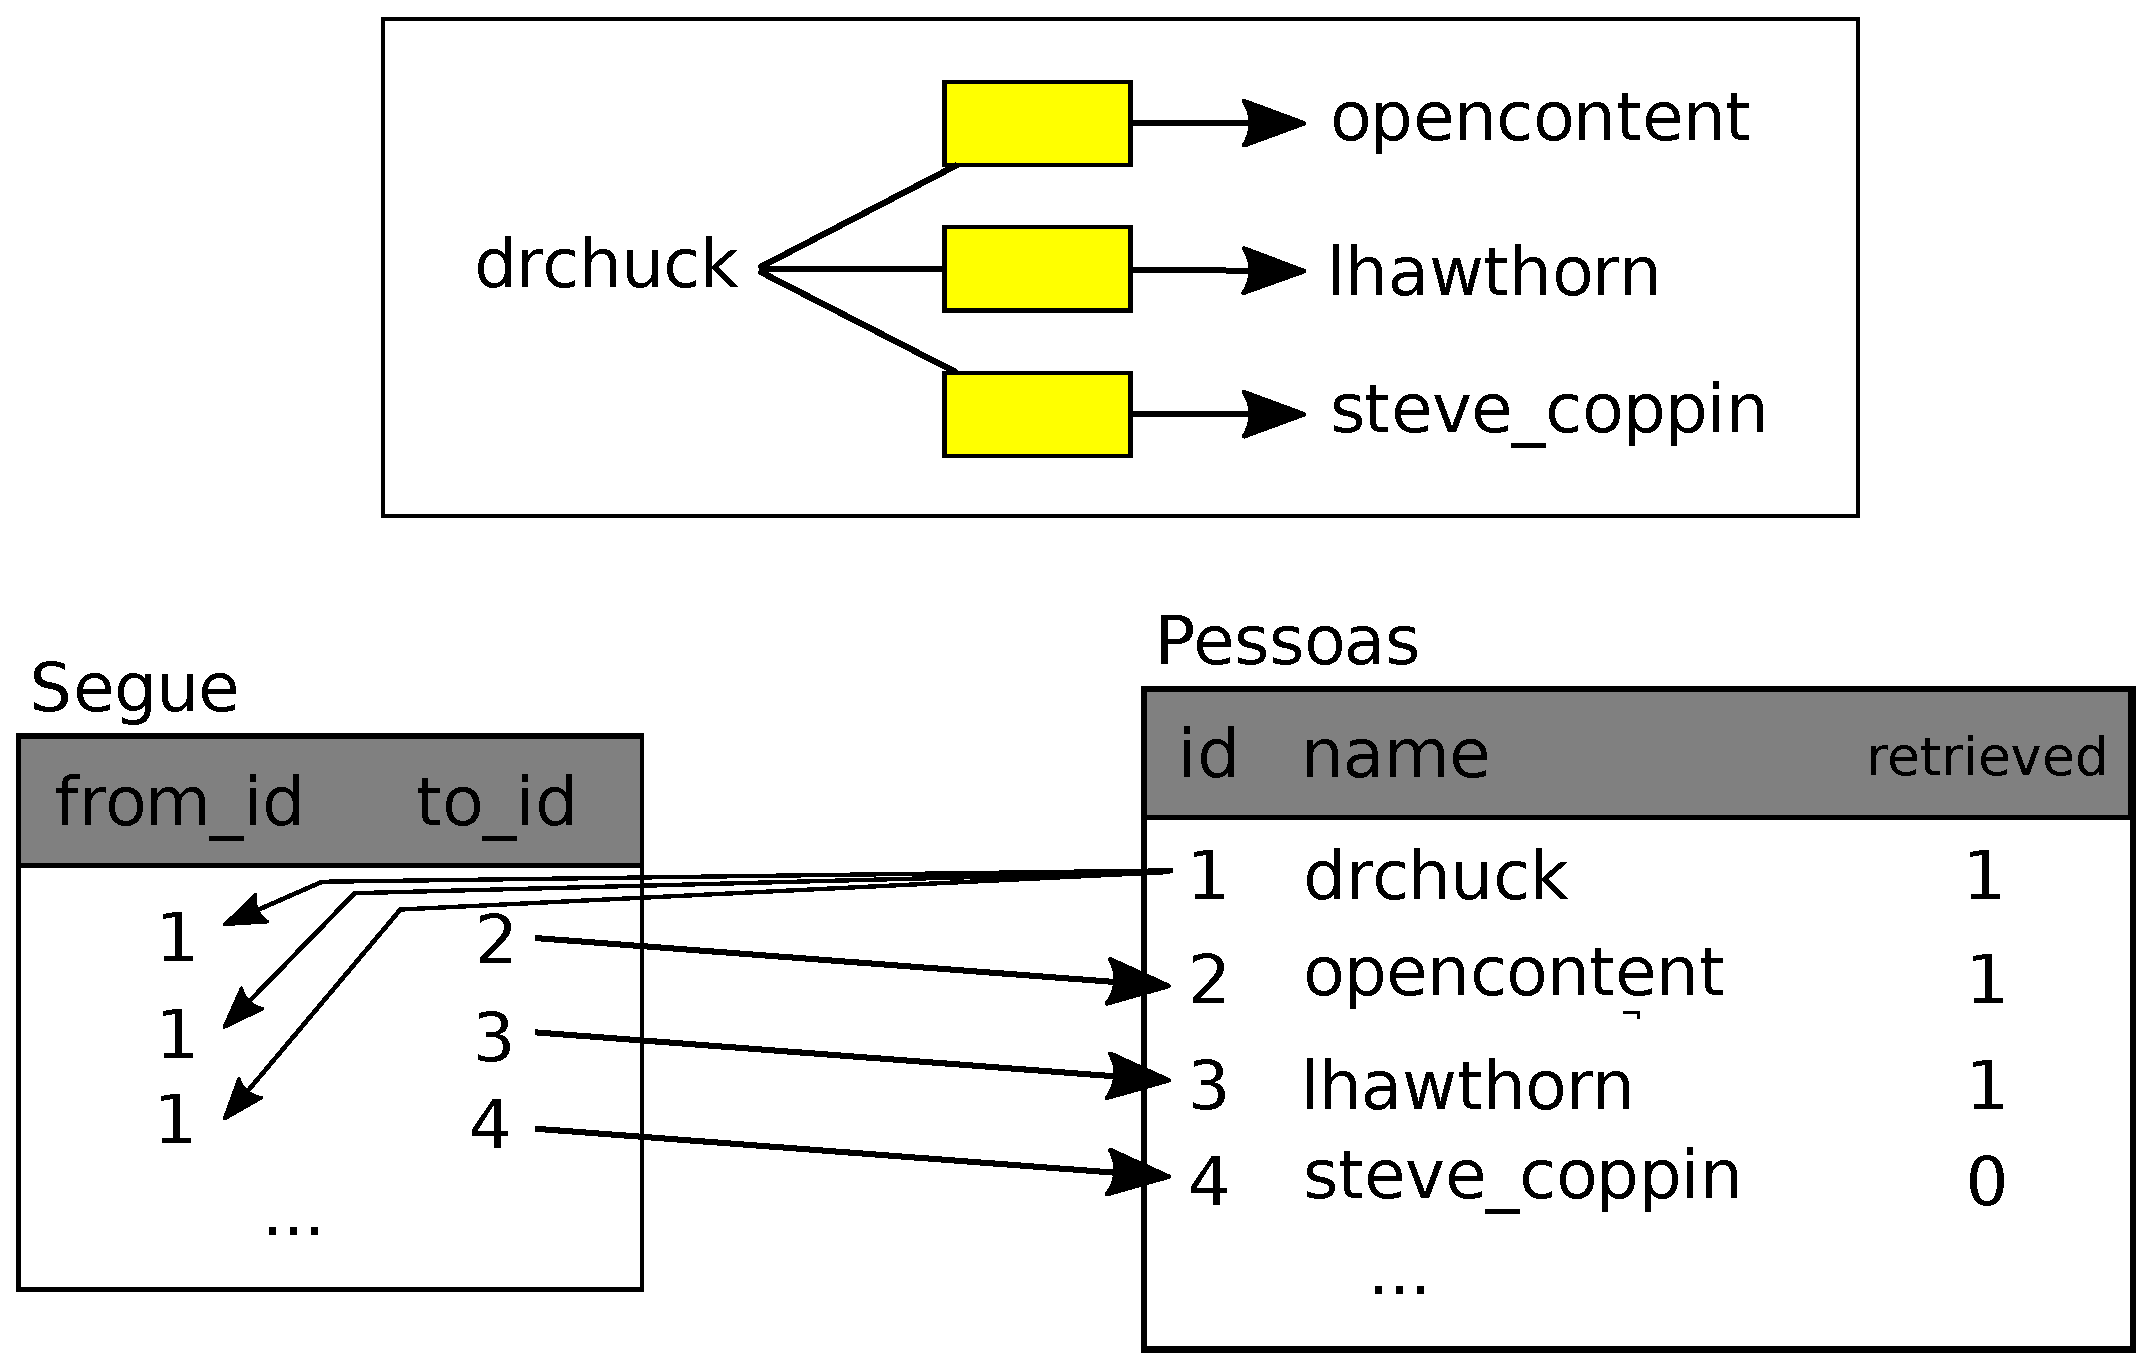
\includegraphics[height=2.50in]{figs2/twitter.eps}}
\afterfig


\section{Programming with multiple tables}

We will now redo the Twitter spider program using two tables, the primary
keys, and the key references as described above.  Here is the code for 
the new version of the program:

\beforeverb
\begin{verbatim}
import urllib
import twurl
import json
import sqlite3

TWITTER_URL = 'https://api.twitter.com/1.1/friends/list.json'

conn = sqlite3.connect('friends.sqlitesqlite3')
cur = conn.cursor()

cur.execute('''CREATE TABLE IF NOT EXISTS People 
    (id INTEGER PRIMARY KEY, name TEXT UNIQUE, retrieved INTEGER)''')
cur.execute('''CREATE TABLE IF NOT EXISTS Follows 
    (from_id INTEGER, to_id INTEGER, UNIQUE(from_id, to_id))''')

while True:
    acct = raw_input('Enter a Twitter account, or quit: ')
    if ( acct == 'quit' ) : break
    if ( len(acct) < 1 ) :
        cur.execute('''SELECT id, name FROM People 
            WHERE retrieved = 0 LIMIT 1''')
        try:
            (id, acct) = cur.fetchone()
        except:
            print 'No unretrieved Twitter accounts found'
            continue
    else:
        cur.execute('SELECT id FROM People WHERE name = ? LIMIT 1', 
            (acct, ) )
        try:
            id = cur.fetchone()[0]
        except:
            cur.execute('''INSERT OR IGNORE INTO People (name, retrieved) 
                VALUES ( ?, 0)''', ( acct, ) )
            conn.commit()
            if cur.rowcount != 1 : 
                print 'Error inserting account:',acct
                continue
            id = cur.lastrowid

    url = twurl.augment(TWITTER_URL, 
       {'screen_name': acct, 'count': '20'} )
    print 'Retrieving account', acct
    connection = urllib.urlopen(url)
    data = connection.read()
    headers = connection.info().dict
    print 'Remaining', headers['x-rate-limit-remaining']

    js = json.loads(data)
    # print json.dumps(js, indent=4)

    cur.execute('UPDATE People SET retrieved=1 WHERE name = ?', (acct, ) )

    countnew = 0
    countold = 0
    for u in js['users'] :
        friend = u['screen_name']
        print friend
        cur.execute('SELECT id FROM People WHERE name = ? LIMIT 1', 
            (friend, ) )
        try:
            friend_id = cur.fetchone()[0]
            countold = countold + 1
        except:
            cur.execute('''INSERT OR IGNORE INTO People (name, retrieved) 
                VALUES ( ?, 0)''', ( friend, ) )
            conn.commit()
            if cur.rowcount != 1 :
                print 'Error inserting account:',friend
                continue
            friend_id = cur.lastrowid
            countnew = countnew + 1
        cur.execute('''INSERT OR IGNORE INTO Follows (from_id, to_id) 
            VALUES (?, ?)''', (id, friend_id) )
    print 'New accounts=',countnew,' revisited=',countold
    conn.commit()

cur.close()
\end{verbatim}
\afterverb
%
This program is starting to get a bit complicated, but it illustrates
the patterns that we need to use when we are
using integer keys to link tables. The basic patterns are:

\begin{enumerate}

\item Create tables with primary keys and constraints.

\item When we have a logical key for a person (i.e., account
name) and we need the {\tt id} value for the person,
depending on whether or not the person is already
in the {\tt People} table we either need to: 
(1) look up the person in the {\tt People} table and 
retrieve the {\tt id} value for the person 
or (2) add the person to the {\tt People} table and get the 
{\tt id} value for the newly added row.

\item Insert the row that captures the ``follows'' relationship.

\end{enumerate}

We will cover each of these in turn.

\subsection{Constraints in database tables}

As we design our table structures, we can tell the database system 
that we would like it to enforce a few rules on us.   These rules
help us from making mistakes and introducing incorrect data into 
out tables.   When we create our tables:

\beforeverb
\begin{verbatim}
cur.execute('''CREATE TABLE IF NOT EXISTS People 
    (id INTEGER PRIMARY KEY, name TEXT UNIQUE, retrieved INTEGER)''')
cur.execute('''CREATE TABLE IF NOT EXISTS Follows 
    (from_id INTEGER, to_id INTEGER, UNIQUE(from_id, to_id))''')
\end{verbatim}
\afterverb
%
We indicate that the {\tt name} column in the {\tt People} table must be
{\tt UNIQUE}.   We also indicate that the combination of the two numbers
in each row of the {\tt Follows} table must be unique.  These constraints
keep us from making mistakes such as adding the same relationship more than
once.

We can take advantage of these constraints in the following code:

\beforeverb
\begin{verbatim}
cur.execute('''INSERT OR IGNORE INTO People (name, retrieved) 
    VALUES ( ?, 0)''', ( friend, ) )
\end{verbatim}
\afterverb
%
We add the {\tt OR IGNORE} clause to our {\tt INSERT} statement to indicate
that if this particular {\tt INSERT} would cause a violation of the
``{\tt name} must be unique'' rule, the database system is allowed to ignore the 
{\tt INSERT}.  We are using the database constraint as a safety net
to make sure we don't inadvertently do something incorrect.

Similarly, the following code ensures that we don't add the 
exact same {\tt Follows} relationship twice.

\beforeverb
\begin{verbatim}
cur.execute('''INSERT OR IGNORE INTO Follows 
    (from_id, to_id) VALUES (?, ?)''', (id, friend_id) )
\end{verbatim}
\afterverb
%
Again, we simply tell the database to ignore our attempted 
{\tt INSERT} if it would violate the uniqueness constraint
that we specified for the {\tt Follows} rows.

\subsection{Retrieve and/or insert a record}

When we prompt the user for a Twitter account, if the account 
exists, we must look up its {\tt id} value.  If the account
does not yet exist in the {\tt People} table, we must insert 
the record and get the {\tt id} value from the inserted
row.

This is a very common pattern and is done twice in the program above.
This code shows how we look up the {\tt id} for a 
friend's account when we have extracted a \verb"screen_name"
from a {\tt user} node in the retrieved Twitter JSON.

Since over time it will be increasingly likely that the account
will already be in the database, we first check to see if the
{\tt People} record exists using a {\tt SELECT} statement.

If all goes well\footnote{In general, when a sentence starts 
with ``if all goes well'' you will find that the code needs
to use try/except.} inside the {\tt try} section, we retrieve the
record using {\tt fetchone()} and then retrieve the
first (and only) element of the returned tuple and store it in 
\verb"friend_id".

If the {\tt SELECT} fails, the {\tt fetchone()[0]} code will fail
and control will transfer into the {\tt except} section.

\beforeverb
\begin{verbatim}
        friend = u['screen_name']
        cur.execute('SELECT id FROM People WHERE name = ? LIMIT 1',
            (friend, ) )
        try:
            friend_id = cur.fetchone()[0]
            countold = countold + 1
        except:
            cur.execute('''INSERT OR IGNORE INTO People (name, retrieved) 
                VALUES ( ?, 0)''', ( friend, ) )
            conn.commit()
            if cur.rowcount != 1 :
                print 'Error inserting account:',friend
                continue
            friend_id = cur.lastrowid
            countnew = countnew + 1
\end{verbatim}
\afterverb
%
If we end up in the {\tt except} code, it simply means that the row
was not found, so we must insert the row.  We use {\tt INSERT OR 
IGNORE} just to avoid errors and then call {\tt commit()} to 
force the database to really be updated.  After the write is done, we can 
check the {\tt cur.rowcount} to see how many rows were affected.  Since
we are attempting to insert a single row, if the number of 
affected rows is something other than 1, it is an error.  

If the {\tt INSERT} is successful, we can look at {\tt cur.lastrowid} 
to find out what value the database assigned to the {\tt id} column in 
our newly created row.

\subsection{Storing the friend relationship}

Once we know the key value for both the Twitter user
and the friend in the JSON, it is a simple matter to insert
the two numbers into the {\tt Follows} table
with the following code:

\beforeverb
\begin{verbatim}
cur.execute('INSERT OR IGNORE INTO Follows (from_id, to_id) VALUES (?, ?)',
    (id, friend_id) )
\end{verbatim}
\afterverb
%
Notice that we let the database take care of keeping us from ``double-inserting''
a relationship by creating the table with a uniqueness constraint and then
adding {\tt OR IGNORE} to our {\tt INSERT} statement.

Here is a sample execution of this program:

\beforeverb
\begin{verbatim}
Enter a Twitter account, or quit: 
No unretrieved Twitter accounts found
Enter a Twitter account, or quit: drchuck
Retrieving http://api.twitter.com/1.1/friends ...
New accounts= 20  revisited= 0
Enter a Twitter account, or quit: 
Retrieving http://api.twitter.com/1.1/friends ...
New accounts= 17  revisited= 3
Enter a Twitter account, or quit: 
Retrieving http://api.twitter.com/1.1/friends ...
New accounts= 17  revisited= 3
Enter a Twitter account, or quit: quit
\end{verbatim}
\afterverb
%
We started with the {\tt drchuck} account and then let the program
automatically pick the next two accounts to retrieve and add to 
our database.

The following is the first few rows in the {\tt People} 
and {\tt Follows} tables after this run is completed:

\beforeverb
\begin{verbatim}
People:
(1, u'drchuck', 1)
(2, u'opencontent', 1)
(3, u'lhawthorn', 1)
(4, u'steve_coppin', 0)
(5, u'davidkocher', 0)
55 rows.
Follows:
(1, 2)
(1, 3)
(1, 4)
(1, 5)
(1, 6)
60 rows.
\end{verbatim}
\afterverb
%
You can see the {\tt id}, {\tt name}, and {\tt visited} fields in the 
{\tt People} table and you see the numbers of both ends of 
the relationship in the {\tt Follows} table.   
In the {\tt People} table, we can see that the first three people
have been visited and their data has been retrieved.
The data in the {\tt Follows} table indicates that
{\tt drchuck} (user 1) is a friend to all of the people shown in the first
five rows.  This makes sense because
the first data we retrieved and stored was the Twitter friends of
{\tt drchuck}.  If you were to print more rows from the {\tt Follows} table,
you would see the friends of users 2 and 3 as well.

\section{Three kinds of keys}

Now that we have started building a data model putting our
data into multiple linked tables and linking the rows in those
tables using {\bf keys}, we need to look at some terminology 
around keys.  There are generally three kinds of keys used 
in a database model.

\begin{itemize}

\item A {\bf logical key} is a key that the ``real world'' might use
to look up a row.   In our example data model, the {\tt name}
field is a logical key.  It is the screen name for the user 
and we indeed look up a user's row several times in the program
using the {\tt name} field.  You will often find that it makes
sense to add a {\tt UNIQUE} constraint to a logical key.  Since the 
logical key is how we look up a row from the outside world, it makes
little sense to allow multiple rows with the same value in the table.

\item A {\bf primary key} is usually a number that is assigned
automatically by the database.  It generally has no meaning outside
the program and is only used to link rows from different tables
together.  When we want to look up a row in a table, usually 
searching for the row using the primary key is the fastest 
way to find the row.  Since primary keys are integer numbers, they 
take up very little storage and can be compared or sorted very quickly.
In our data model, the {\tt id} field is an example of a primary key.

\item A {\bf foreign key} is usually a number that points to the primary key
of an associated row in a different table.  An example of a foreign
key in our data model is the \verb"from_id".  

\end{itemize}

We are using a
naming convention of always calling the primary key field name
{\tt id} and appending the suffix \verb"_id" to any field name
that is a foreign key.


\section{Using JOIN to retrieve data}

Now that we have followed the rules of database normalization
and have data separated into two tables, linked together using
primary and foreign keys, we need to be able to build a 
{\tt SELECT} that reassembles the data across the tables.

SQL uses the {\tt JOIN} clause to reconnect these tables.  
In the {\tt JOIN} clause you specify the fields that are used 
to reconnect the rows between the tables.

The following is an example of a {\tt SELECT} with a 
{\tt JOIN} clause:

\beforeverb
\begin{verbatim}
SELECT * FROM Follows JOIN People 
    ON Follows.from_id = People.id WHERE People.id = 1
\end{verbatim}
\afterverb
%
The {\tt JOIN} clause indicates that the fields we are selecting
cross both the {\tt Follows} and {\tt People} tables.  The {\tt ON}
clause indicates how the two tables are to be joined:  Take the rows
from {\tt Follows} and append the row from {\tt People} where the
field \verb"from_id" in {\tt Follows} is the same the {\tt id} value
in the {\tt People} table.

\beforefig
\centerline{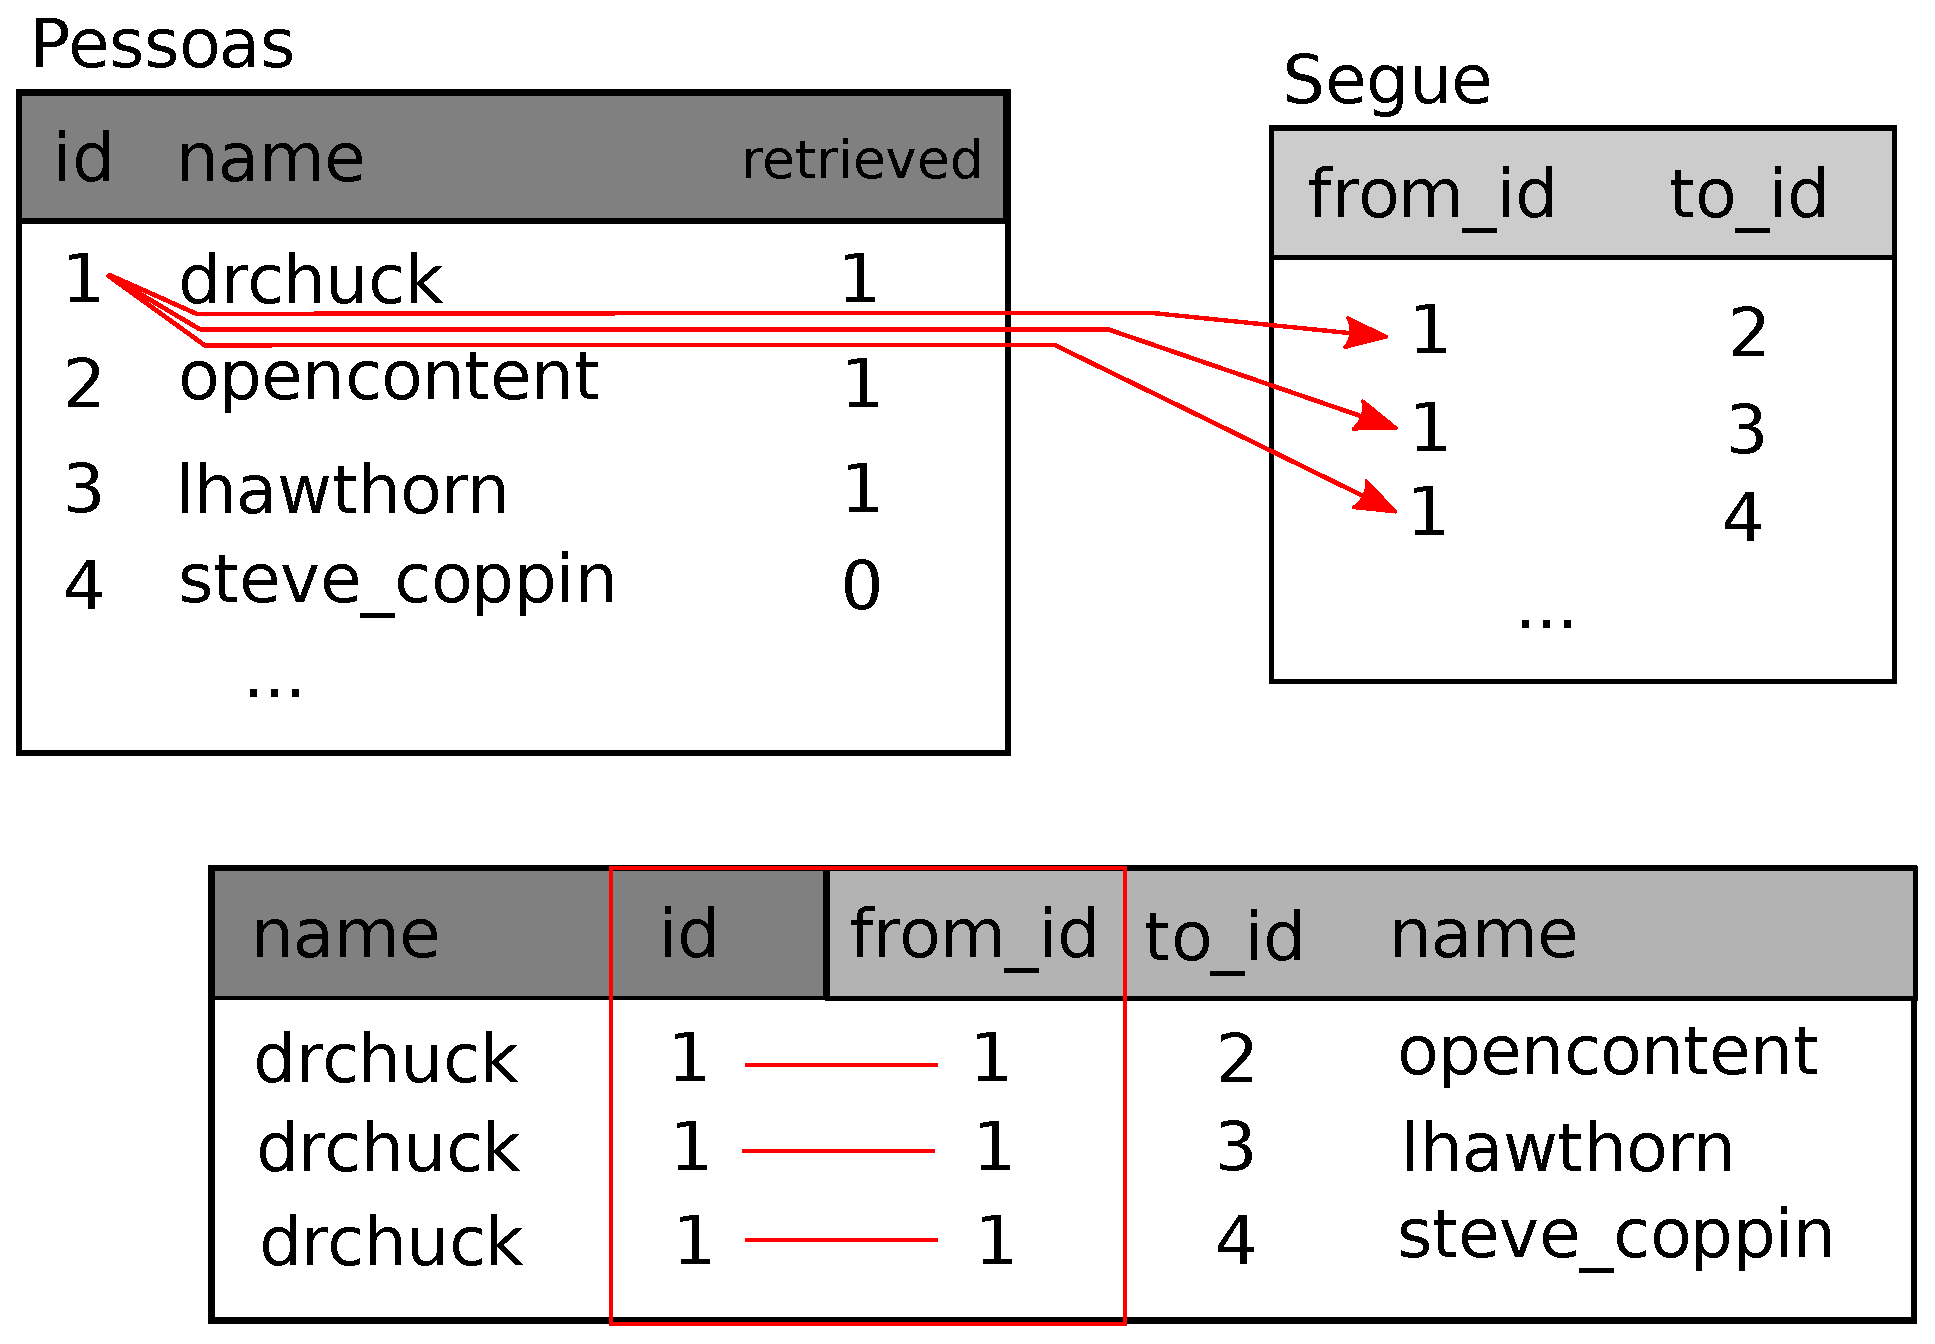
\includegraphics[height=2.50in]{figs2/join.eps}}
\afterfig

The result of the JOIN is to create extra-long ``metarows'' which have both 
the fields from {\tt People} and the matching fields from {\tt Follows}.
Where there is more than one match between the {\tt id} field from {\tt People}
and the \verb"from_id" from {\tt People}, then JOIN creates a metarow 
for \emph{each} of the matching pairs of rows, duplicating data as needed.

The following code demonstrates the data that we will have in the 
database after the multi-table Twitter spider program (above) has
been run several times.

\beforeverb
\begin{verbatim}
import sqlite3

conn = sqlite3.connect('spider.sqlite3')
cur = conn.cursor()

cur.execute('SELECT * FROM People')
count = 0
print 'People:'
for row in cur :
   if count < 5: print row
   count = count + 1
print count, 'rows.'

cur.execute('SELECT * FROM Follows')
count = 0
print 'Follows:'
for row in cur :
   if count < 5: print row
   count = count + 1
print count, 'rows.'

cur.execute('''SELECT * FROM Follows JOIN People 
    ON Follows.to_id = People.id WHERE Follows.from_id = 2''')
count = 0
print 'Connections for id=2:'
for row in cur :
   if count < 5: print row
   count = count + 1
print count, 'rows.'

cur.close()
\end{verbatim}
\afterverb
%
In this program, we first dump out the {\tt People}
and {\tt Follows} and then dump out a subset of the
data in the tables joined together.

Here is the output of the program:

\beforeverb
\begin{verbatim}
python twjoin.py 
People:
(1, u'drchuck', 1)
(2, u'opencontent', 1)
(3, u'lhawthorn', 1)
(4, u'steve_coppin', 0)
(5, u'davidkocher', 0)
55 rows.
Follows:
(1, 2)
(1, 3)
(1, 4)
(1, 5)
(1, 6)
60 rows.
Connections for id=2:
(2, 1, 1, u'drchuck', 1)
(2, 28, 28, u'cnxorg', 0)
(2, 30, 30, u'kthanos', 0)
(2, 102, 102, u'SomethingGirl', 0)
(2, 103, 103, u'ja_Pac', 0)
20 rows.
\end{verbatim}
\afterverb
%
You see the columns from the {\tt People} and {\tt Follows} tables and the last
set of rows is the result of the {\tt SELECT} with the {\tt JOIN} clause.

In the last select, we are looking for accounts that are friends of 
``opencontent'' (i.e., {\tt People.id=2}).

In each of the ``metarows'' in the last select, the first two columns are
from the {\tt Follows}
table followed by columns three through five from the {\tt People} table.  You can also
see that the second column (\verb"Follows.to_id") matches the third column
({\tt People.id}) in each of the joined-up ``metarows''.

\section{Summary}

This chapter has covered a lot of ground to give you an overview of the basics
of using a database in Python.   It is more complicated to write the code to use 
a database to store data than Python dictionaries or flat files so there is 
little reason to use a database unless your application truly needs the capabilities
of a database.  The situations where a database can be quite useful are: 
(1) when your application needs to make small many random updates within a large data set,
(2) when your data is so large it cannot fit in a dictionary and you need to 
look up information repeatedly, or (3) when you have a long-running process that you
want to be able to stop and restart and retain the data from one run to the next.

You can build a simple database with a single table to suit many application 
needs, but most problems will require several tables and links/relationships
between rows in different tables.   When you start making links between 
tables, it is important to do some thoughtful design and follow the 
rules of database normalization to make the best use of the database's
capabilities.  Since the primary motivation for using a database
is that you have a large amount of data to deal with, it is important
to model your data efficiently so your programs run as fast as possible.

\section{Debugging}

One common pattern when you are developing a Python program to connect to
an SQLite database will be to run a Python program and check the
results using the SQLite Database Browser.  The browser allows you 
to quickly check to see if your program is working properly.

You must be careful because SQLite takes care to keep two programs
from changing the same data at the same time.   For example, if
you open a database in the browser and make a change to the database
and have not yet pressed the ``save'' button in the browser, the 
browser ``locks'' the database file and keeps any other program
from accessing the file.  In particular, your Python program
will not be able to access the file if it is locked.

So a solution is to make sure to either close the database browser 
or use the {\bf File} menu to close the database in the browser
before you attempt to access the database from Python to avoid
the problem of your Python code failing because the database is
locked.

\section{Glossary}

\begin{description}

\item[attribute:] One of the values within a tuple.  More commonly
called a ``column'' or ``field''.
\index{attribute}

\item[constraint:] 
When we tell the database to enforce a rule on a field or a row
in a table.  A common constraint is to insist that there can be no
duplicate values in a particular field (i.e., all the values must be unique).
\index{constraint}

\item[cursor:] A cursor allows you to execute SQL commands in a database
and retrieve data from the database.  A cursor is similar to 
a socket or file handle for network connections and files, respectively.
\index{cursor}

\item[database browser:] 
A piece of software that allows you to directly connect to a database 
and manipulate the database directly without writing a program.
\index{database browser}

\item[foreign key:] A numeric key that points to the primary key of 
a row in another table.  Foreign keys establish relationships between rows
stored in different tables.
\index{foreign key}

\item[index:] Additional data that the database software maintains as rows
and inserts into a table to make lookups very fast.
\index{index}

\item[logical key:] A key that the ``outside world'' uses to look up a particular
row.  For example in a table of user accounts, a person's email address
might be a good candidate as the logical key for the user's data. 
\index{logical key}

\item[normalization:] Designing a data model so that no data
is replicated.  We store each item of data at one place in the database
and reference it elsewhere using a foreign key.
\index{normalization}
\index{database normalization}

\item[primary key:] A numeric key assigned to each row that is used to 
refer to one row in a table from another table.  Often the database
is configured to automatically assign primary keys as rows are inserted.
\index{primary key}

\item[relation:] An area within a database that contains tuples and 
attributes.  More typically called a ``table''.
\index{relation}

\item[tuple:] A single entry in a database table that is a set 
of attributes.  More typically called ``row''.
\index{tuple}

\end{description}


% TODO \input{15-viz}
% TODO \input{16-tasks}

\appendix

% TODO \input{AA-windows}
% TODO \input{AB-apple}
% TODO \input{AC-contrib}
% TODO \input{AD-copyright}

\normalsize

\printindex

\clearemptydoublepage

\end{document}
